\documentclass[10pt]{report}
\usepackage{graphicx}
\parindent=0in
\textwidth=6.7in 
\textheight=9in
\setlength{\oddsidemargin}{-0.10in}
\setlength{\evensidemargin}{-0.10in}
\setlength{\topmargin}{-0.55in}
\setlength{\unitlength}{0.5in}
\pagestyle{empty}

\begin{document}

\begin{center}
{\large Instituto Tecnol\'{o}gico y de Estudios Superiores de Monterrey \\
An\'alisis Estad\'stico de Datos } \\
Examen Argumentativo (Papel)
\end{center}

Nombre: \underline{\hspace*{.2in}}
Adriana Pérez
\underline{\hspace*{.2in}} \quad Matr\'icula:\underline{\hspace*{.2in}}
A00000001
\underline{\hspace*{.2in}} \\

{\bf Instrucciones:} Lee con cuidado cada problema y escribe la soluci\'on
en tu hoja de respuesta. Incluye tu procedimiento que muestre c\'omo obtienes tu respuesta.  Respeta el c\'odigo de \'etica del curso y del Tecnol\'ogico de Monterrey y responde los ejercicios de manera individual sin ayuda externa o no autorizada.

\begin{enumerate}

\item Una empresa que fabrica l\'aminas de aluminio para la industria aeron\'autica necesita asegurar que el espesor de sus l\'aminas cumple con las especificaciones de $2.5 \pm 0.1$ mm. Se ha implementado una nueva maquinaria y se desea monitorear el espesor de las l\'aminas. Para ello, se han tomado muestras de tama\~no 5 cada hora y se gener\'o el diagrama que se muestra abajo.
\begin{enumerate}
\item (5 pts) Calcula la media y variabilidad del proceso (dentro de grupos).
\item (10 pts) Calcula los l\'imites de control para la {\bf variabilidad} del espesor de las láminas.
\item (10 pts) Calcula el porcentaje de l\'aminas que tienen un espesor menor a 2.4 mm. Use los valores del inciso a) para calcular este porcentaje.
\end{enumerate}
\begin{figure}[h!]
\centering
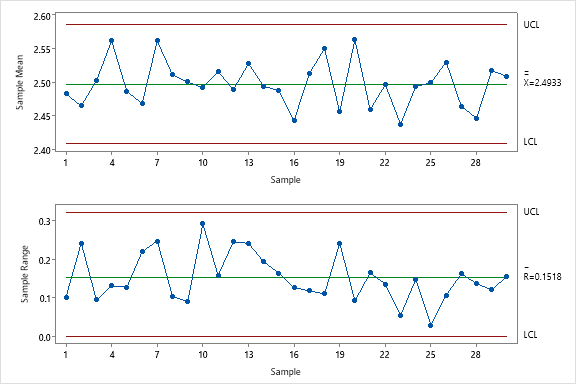
\includegraphics[width=0.75\textwidth]{Xbar_R_Paper.png}
\end{figure}


\item Una empresa que fabrica tarjetas de circuitos impresos desea evaluar si la implementaci\'on de un nuevo sistema de ensamblaje ha reducido el n\'umero de disconformidades. Se tomaron 50 mediciones, antes y después del cambio, para analizar los efectos.
\begin{center}
\begin{tabular}{|l|c|c|}
\hline
 & Antes & Después \\ 
\hline
Media muestral & 3.60 & 2.37 \\ 
\hline
Desviaci'on est'andar muestral & 1.09 & 1.62 \\ 
\hline
\end{tabular}
\end{center}
\begin{enumerate}
\item (15 pts) Calcula un intervalo de confianza de 90\% para el número medio de disconformidades antes del cambio.
\item (15 pts) Calcula un intervalo de confianza de 90\% para la estimar la diferencia en el número medio de disconformidades antes y después del cambio. ¿Qu\'e puedes concluir con este resultado?
\end{enumerate}


\end{enumerate}
  
\newpage



\begin{center}
{\large Instituto Tecnol\'{o}gico y de Estudios Superiores de Monterrey \\
An\'alisis Estad\'stico de Datos } \\
Examen Argumentativo (Papel)
\end{center}

Nombre: \underline{\hspace*{.2in}}
Fernando López
\underline{\hspace*{.2in}} \quad Matr\'icula:\underline{\hspace*{.2in}}
A00000002
\underline{\hspace*{.2in}} \\

{\bf Instrucciones:} Lee con cuidado cada problema y escribe la soluci\'on
en tu hoja de respuesta. Incluye tu procedimiento que muestre c\'omo obtienes tu respuesta.  Respeta el c\'odigo de \'etica del curso y del Tecnol\'ogico de Monterrey y responde los ejercicios de manera individual sin ayuda externa o no autorizada.

\begin{enumerate}

\item Una empresa que fabrica l\'aminas de aluminio para la industria aeron\'autica necesita asegurar que el espesor de sus l\'aminas cumple con las especificaciones de $2.5 \pm 0.1$ mm. Se ha implementado una nueva maquinaria y se desea monitorear el espesor de las l\'aminas. Para ello, se han tomado muestras de tama\~no 4 cada hora y se gener\'o el diagrama que se muestra abajo.
\begin{enumerate}
\item (5 pts) Calcula la media y variabilidad del proceso (dentro de grupos).
\item (10 pts) Calcula los l\'imites de control para la {\bf variabilidad} del espesor de las láminas.
\item (10 pts) Calcula el porcentaje de l\'aminas que tienen un espesor mayor a 2.6 mm. Use los valores del inciso a) para calcular este porcentaje.
\end{enumerate}
\begin{figure}[h!]
\centering
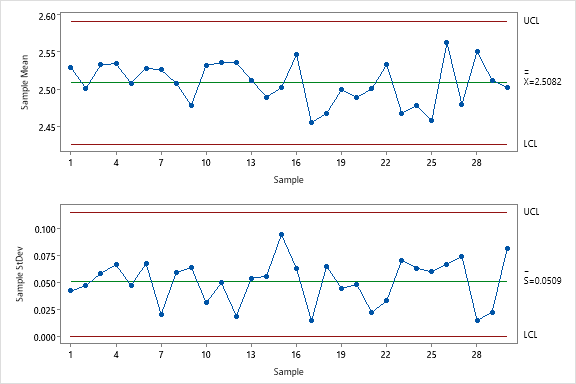
\includegraphics[width=0.75\textwidth]{Xbar_S_Paper.png}
\end{figure}


\item Una empresa que fabrica tarjetas de circuitos impresos desea evaluar si la implementaci\'on de un nuevo sistema de ensamblaje ha reducido el n\'umero de disconformidades. Se tomaron 50 mediciones, antes y después del cambio, para analizar los efectos.
\begin{center}
\begin{tabular}{|l|c|c|}
\hline
 & Antes & Después \\ 
\hline
Media muestral & 3.60 & 2.37 \\ 
\hline
Desviaci'on est'andar muestral & 1.09 & 1.62 \\ 
\hline
\end{tabular}
\end{center}
\begin{enumerate}
\item (15 pts) Calcula un intervalo de confianza de 90\% para el número medio de disconformidades antes del cambio.
\item (15 pts) ¿Existe suficiente evidencia para concluir que el número medio de disconformidades ha disminuido despu\'es del cambio? Usa un nivel de significancia de 0.05.
\end{enumerate}


\end{enumerate}
  
\newpage



\begin{center}
{\large Instituto Tecnol\'{o}gico y de Estudios Superiores de Monterrey \\
An\'alisis Estad\'stico de Datos } \\
Examen Argumentativo (Papel)
\end{center}

Nombre: \underline{\hspace*{.2in}}
Karen Rodríguez
\underline{\hspace*{.2in}} \quad Matr\'icula:\underline{\hspace*{.2in}}
A00000003
\underline{\hspace*{.2in}} \\

{\bf Instrucciones:} Lee con cuidado cada problema y escribe la soluci\'on
en tu hoja de respuesta. Incluye tu procedimiento que muestre c\'omo obtienes tu respuesta.  Respeta el c\'odigo de \'etica del curso y del Tecnol\'ogico de Monterrey y responde los ejercicios de manera individual sin ayuda externa o no autorizada.

\begin{enumerate}

\item Una empresa que fabrica l\'aminas de aluminio para la industria aeron\'autica necesita asegurar que el espesor de sus l\'aminas cumple con las especificaciones de $2.5 \pm 0.1$ mm. Se ha implementado una nueva maquinaria y se desea monitorear el espesor de las l\'aminas. Para ello, se han tomado muestras de tama\~no 5 cada hora y se gener\'o el diagrama que se muestra abajo.
\begin{enumerate}
\item (5 pts) Calcula la media y variabilidad del proceso (dentro de grupos).
\item (10 pts) Calcula los l\'imites de control para la {\bf variabilidad} del espesor de las láminas.
\item (10 pts) Calcula el porcentaje de l\'aminas que tienen un espesor menor a 2.4 mm. Use los valores del inciso a) para calcular este porcentaje.
\end{enumerate}
\begin{figure}[h!]
\centering
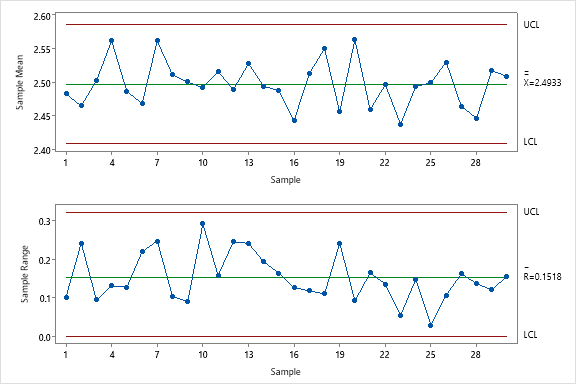
\includegraphics[width=0.75\textwidth]{Xbar_R_Paper.png}
\end{figure}


\item Una empresa que fabrica tarjetas de circuitos impresos desea evaluar si la implementaci\'on de un nuevo sistema de ensamblaje ha reducido el n\'umero de disconformidades. Se tomaron 50 mediciones, antes y después del cambio, para analizar los efectos.
\begin{center}
\begin{tabular}{|l|c|c|}
\hline
 & Antes & Después \\ 
\hline
Media muestral & 3.60 & 2.37 \\ 
\hline
Desviaci'on est'andar muestral & 1.09 & 1.62 \\ 
\hline
\end{tabular}
\end{center}
\begin{enumerate}
\item (15 pts) Calcula un intervalo de confianza de 90\% para el número medio de disconformidades antes del cambio.
\item (15 pts) Calcula un intervalo de confianza de 90\% para la estimar la diferencia en el número medio de disconformidades antes y después del cambio. ¿Qu\'e puedes concluir con este resultado?
\end{enumerate}


\end{enumerate}
  
\newpage



\begin{center}
{\large Instituto Tecnol\'{o}gico y de Estudios Superiores de Monterrey \\
An\'alisis Estad\'stico de Datos } \\
Examen Argumentativo (Papel)
\end{center}

Nombre: \underline{\hspace*{.2in}}
Óscar Mendoza
\underline{\hspace*{.2in}} \quad Matr\'icula:\underline{\hspace*{.2in}}
A00000004
\underline{\hspace*{.2in}} \\

{\bf Instrucciones:} Lee con cuidado cada problema y escribe la soluci\'on
en tu hoja de respuesta. Incluye tu procedimiento que muestre c\'omo obtienes tu respuesta.  Respeta el c\'odigo de \'etica del curso y del Tecnol\'ogico de Monterrey y responde los ejercicios de manera individual sin ayuda externa o no autorizada.

\begin{enumerate}

\item Una empresa que fabrica l\'aminas de aluminio para la industria aeron\'autica necesita asegurar que el espesor de sus l\'aminas cumple con las especificaciones de $2.5 \pm 0.1$ mm. Se ha implementado una nueva maquinaria y se desea monitorear el espesor de las l\'aminas. Para ello, se han tomado muestras de tama\~no 4 cada hora y se gener\'o el diagrama que se muestra abajo.
\begin{enumerate}
\item (5 pts) Calcula la media y variabilidad del proceso (dentro de grupos).
\item (10 pts) Calcula los l\'imites de control para el espesor de las láminas.
\item (10 pts) Calcula el porcentaje de l\'aminas que cumplen con las especificaciones. Use los valores del inciso a) para calcular este porcentaje.
\end{enumerate}
\begin{figure}[h!]
\centering
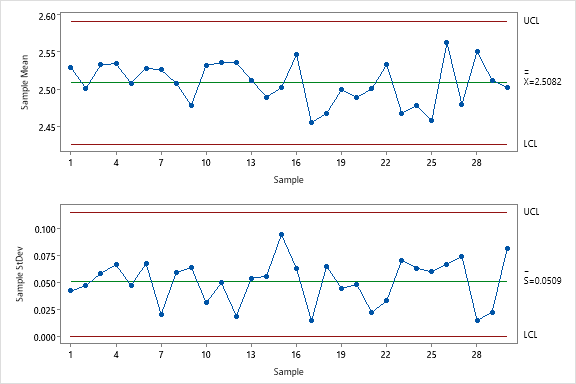
\includegraphics[width=0.75\textwidth]{Xbar_S_Paper.png}
\end{figure}


\item Una empresa que fabrica tarjetas de circuitos impresos desea evaluar si la implementaci\'on de un nuevo sistema de ensamblaje ha reducido el n\'umero de disconformidades. Se tomaron 50 mediciones, antes y después del cambio, para analizar los efectos.
\begin{center}
\begin{tabular}{|l|c|c|}
\hline
 & Antes & Después \\ 
\hline
Media muestral & 3.60 & 2.37 \\ 
\hline
Desviaci'on est'andar muestral & 1.09 & 1.62 \\ 
\hline
\end{tabular}
\end{center}
\begin{enumerate}
\item (15 pts) Calcula un intervalo de confianza de 90\% para el número medio de disconformidades antes del cambio.
\item (15 pts) Calcula un intervalo de confianza de 90\% para la estimar la diferencia en el número medio de disconformidades antes y después del cambio. ¿Qu\'e puedes concluir con este resultado?
\end{enumerate}


\end{enumerate}
  
\newpage



\begin{center}
{\large Instituto Tecnol\'{o}gico y de Estudios Superiores de Monterrey \\
An\'alisis Estad\'stico de Datos } \\
Examen Argumentativo (Papel)
\end{center}

Nombre: \underline{\hspace*{.2in}}
Melissa Castro
\underline{\hspace*{.2in}} \quad Matr\'icula:\underline{\hspace*{.2in}}
A00000005
\underline{\hspace*{.2in}} \\

{\bf Instrucciones:} Lee con cuidado cada problema y escribe la soluci\'on
en tu hoja de respuesta. Incluye tu procedimiento que muestre c\'omo obtienes tu respuesta.  Respeta el c\'odigo de \'etica del curso y del Tecnol\'ogico de Monterrey y responde los ejercicios de manera individual sin ayuda externa o no autorizada.

\begin{enumerate}

\item Una empresa que fabrica l\'aminas de aluminio para la industria aeron\'autica necesita asegurar que el espesor de sus l\'aminas cumple con las especificaciones de $2.5 \pm 0.1$ mm. Se ha implementado una nueva maquinaria y se desea monitorear el espesor de las l\'aminas. Para ello, se han tomado muestras de tama\~no 4 cada hora y se gener\'o el diagrama que se muestra abajo.
\begin{enumerate}
\item (5 pts) Calcula la media y variabilidad del proceso (dentro de grupos).
\item (10 pts) Calcula los l\'imites de control para el espesor de las láminas.
\item (10 pts) Calcula el porcentaje de l\'aminas que cumplen con las especificaciones. Use los valores del inciso a) para calcular este porcentaje.
\end{enumerate}
\begin{figure}[h!]
\centering
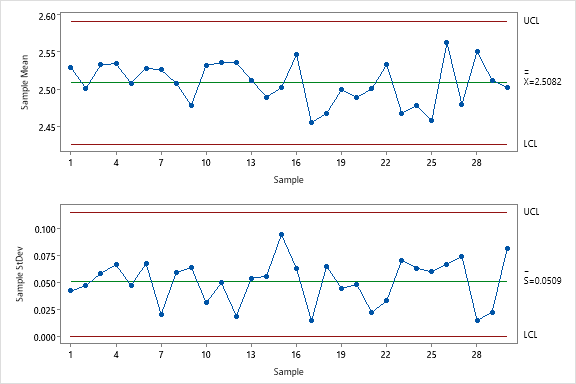
\includegraphics[width=0.75\textwidth]{Xbar_S_Paper.png}
\end{figure}


\item Una empresa que fabrica tarjetas de circuitos impresos desea evaluar si la implementaci\'on de un nuevo sistema de ensamblaje ha reducido el n\'umero de disconformidades. Se tomaron 50 mediciones, antes y después del cambio, para analizar los efectos.
\begin{center}
\begin{tabular}{|l|c|c|}
\hline
 & Antes & Después \\ 
\hline
Media muestral & 3.60 & 2.37 \\ 
\hline
Desviaci'on est'andar muestral & 1.09 & 1.62 \\ 
\hline
\end{tabular}
\end{center}
\begin{enumerate}
\item (15 pts) Calcula un intervalo de confianza de 90\% para el número medio de disconformidades antes del cambio.
\item (15 pts) ¿Existe suficiente evidencia para concluir que el número medio de disconformidades ha disminuido despu\'es del cambio? Usa un nivel de significancia de 0.05.
\end{enumerate}


\end{enumerate}
  
\newpage



\begin{center}
{\large Instituto Tecnol\'{o}gico y de Estudios Superiores de Monterrey \\
An\'alisis Estad\'stico de Datos } \\
Examen Argumentativo (Papel)
\end{center}

Nombre: \underline{\hspace*{.2in}}
Eduardo Vargas
\underline{\hspace*{.2in}} \quad Matr\'icula:\underline{\hspace*{.2in}}
A00000006
\underline{\hspace*{.2in}} \\

{\bf Instrucciones:} Lee con cuidado cada problema y escribe la soluci\'on
en tu hoja de respuesta. Incluye tu procedimiento que muestre c\'omo obtienes tu respuesta.  Respeta el c\'odigo de \'etica del curso y del Tecnol\'ogico de Monterrey y responde los ejercicios de manera individual sin ayuda externa o no autorizada.

\begin{enumerate}

\item En una l\'inea de producci\'on de ejes para motores, el di\'ametro es una caracter\'istica crítica para el ensamblaje adecuado. Las especificaciones del di\'ametro son $50 \pm 0.5$ mm. Se mide el di\'ametro de un eje cada 30 minutos. Despu\'es de 15 horas de mediciones, se obtuvo el gr\'afico IMR con un promedio m\'ovil de orden 2 que se muestra abajo.
\begin{enumerate}
\item (5 pts) Calcula la media y variabilidad del proceso (dentro de grupos).
\item (10 pts) Calcula los l\'imites de control para el di\'ametro del eje.
\item (10 pts) Calcula el porcentaje de ejes que no cumplen con las especificaciones. Use los valores del inciso a) para calcular este porcentaje.
\end{enumerate}
\begin{figure}[h!]
\centering
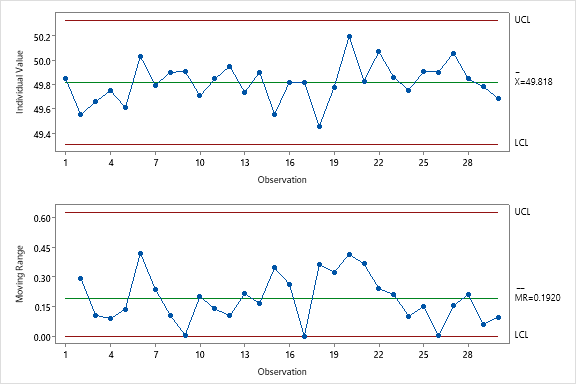
\includegraphics[width=0.75\textwidth]{IMR_Paper.png}
\end{figure}


\item Una empresa que fabrica tarjetas de circuitos impresos desea evaluar si la implementaci\'on de un nuevo sistema de ensamblaje ha reducido el n\'umero de disconformidades. Se tomaron 50 mediciones, antes y después del cambio, para analizar los efectos.
\begin{center}
\begin{tabular}{|l|c|c|}
\hline
 & Antes & Después \\ 
\hline
Media muestral & 3.60 & 2.37 \\ 
\hline
Desviaci'on est'andar muestral & 1.09 & 1.62 \\ 
\hline
\end{tabular}
\end{center}
\begin{enumerate}
\item (15 pts) Calcula un intervalo de confianza de 90\% para el número medio de disconformidades antes del cambio.
\item (15 pts) ¿Existe suficiente evidencia para concluir que el número medio de disconformidades ha disminuido despu\'es del cambio? Usa un nivel de significancia de 0.05.
\end{enumerate}


\end{enumerate}
  
\newpage



\begin{center}
{\large Instituto Tecnol\'{o}gico y de Estudios Superiores de Monterrey \\
An\'alisis Estad\'stico de Datos } \\
Examen Argumentativo (Papel)
\end{center}

Nombre: \underline{\hspace*{.2in}}
Gabriela Núñez
\underline{\hspace*{.2in}} \quad Matr\'icula:\underline{\hspace*{.2in}}
A00000007
\underline{\hspace*{.2in}} \\

{\bf Instrucciones:} Lee con cuidado cada problema y escribe la soluci\'on
en tu hoja de respuesta. Incluye tu procedimiento que muestre c\'omo obtienes tu respuesta.  Respeta el c\'odigo de \'etica del curso y del Tecnol\'ogico de Monterrey y responde los ejercicios de manera individual sin ayuda externa o no autorizada.

\begin{enumerate}

\item Una empresa que fabrica l\'aminas de aluminio para la industria aeron\'autica necesita asegurar que el espesor de sus l\'aminas cumple con las especificaciones de $2.5 \pm 0.1$ mm. Se ha implementado una nueva maquinaria y se desea monitorear el espesor de las l\'aminas. Para ello, se han tomado muestras de tama\~no 4 cada hora y se gener\'o el diagrama que se muestra abajo.
\begin{enumerate}
\item (5 pts) Calcula la media y variabilidad del proceso (dentro de grupos).
\item (10 pts) Calcula los l\'imites de control para la {\bf variabilidad} del espesor de las láminas.
\item (10 pts) Calcula el porcentaje de l\'aminas que tienen un espesor mayor a 2.6 mm. Use los valores del inciso a) para calcular este porcentaje.
\end{enumerate}
\begin{figure}[h!]
\centering
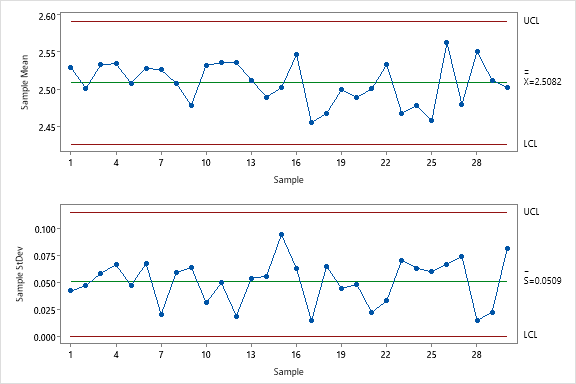
\includegraphics[width=0.75\textwidth]{Xbar_S_Paper.png}
\end{figure}


\item Una empresa que fabrica tarjetas de circuitos impresos desea evaluar si la implementaci\'on de un nuevo sistema de ensamblaje ha reducido el n\'umero de disconformidades. Se tomaron 50 mediciones, antes y después del cambio, para analizar los efectos.
\begin{center}
\begin{tabular}{|l|c|c|}
\hline
 & Antes & Después \\ 
\hline
Media muestral & 3.60 & 2.37 \\ 
\hline
Desviaci'on est'andar muestral & 1.09 & 1.62 \\ 
\hline
\end{tabular}
\end{center}
\begin{enumerate}
\item (15 pts) Calcula un intervalo de confianza de 90\% para el número medio de disconformidades antes del cambio.
\item (15 pts) ¿Existe suficiente evidencia para concluir que el número medio de disconformidades ha disminuido despu\'es del cambio? Usa un nivel de significancia de 0.05.
\end{enumerate}


\end{enumerate}
  
\newpage



\begin{center}
{\large Instituto Tecnol\'{o}gico y de Estudios Superiores de Monterrey \\
An\'alisis Estad\'stico de Datos } \\
Examen Argumentativo (Papel)
\end{center}

Nombre: \underline{\hspace*{.2in}}
Iván Ramírez
\underline{\hspace*{.2in}} \quad Matr\'icula:\underline{\hspace*{.2in}}
A00000008
\underline{\hspace*{.2in}} \\

{\bf Instrucciones:} Lee con cuidado cada problema y escribe la soluci\'on
en tu hoja de respuesta. Incluye tu procedimiento que muestre c\'omo obtienes tu respuesta.  Respeta el c\'odigo de \'etica del curso y del Tecnol\'ogico de Monterrey y responde los ejercicios de manera individual sin ayuda externa o no autorizada.

\begin{enumerate}

\item Una empresa que fabrica l\'aminas de aluminio para la industria aeron\'autica necesita asegurar que el espesor de sus l\'aminas cumple con las especificaciones de $2.5 \pm 0.1$ mm. Se ha implementado una nueva maquinaria y se desea monitorear el espesor de las l\'aminas. Para ello, se han tomado muestras de tama\~no 4 cada hora y se gener\'o el diagrama que se muestra abajo.
\begin{enumerate}
\item (5 pts) Calcula la media y variabilidad del proceso (dentro de grupos).
\item (10 pts) Calcula los l\'imites de control para el espesor de las láminas.
\item (10 pts) Calcula el porcentaje de l\'aminas que cumplen con las especificaciones. Use los valores del inciso a) para calcular este porcentaje.
\end{enumerate}
\begin{figure}[h!]
\centering
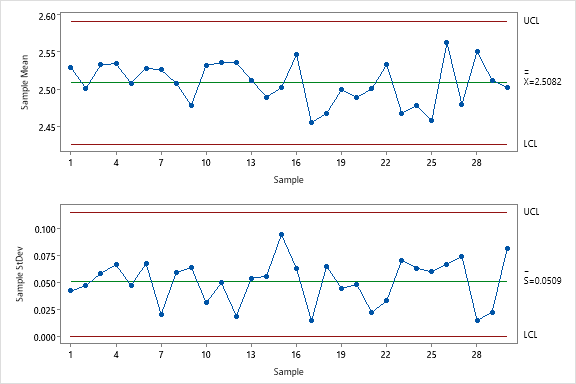
\includegraphics[width=0.75\textwidth]{Xbar_S_Paper.png}
\end{figure}


\item Una empresa que fabrica tarjetas de circuitos impresos desea evaluar si la implementaci\'on de un nuevo sistema de ensamblaje ha reducido el n\'umero de disconformidades. Se tomaron 50 mediciones, antes y después del cambio, para analizar los efectos.
\begin{center}
\begin{tabular}{|l|c|c|}
\hline
 & Antes & Después \\ 
\hline
Media muestral & 3.60 & 2.37 \\ 
\hline
Desviaci'on est'andar muestral & 1.09 & 1.62 \\ 
\hline
\end{tabular}
\end{center}
\begin{enumerate}
\item (15 pts) Calcula un intervalo de confianza de 90\% para el número medio de disconformidades antes del cambio.
\item (15 pts) ¿Existe suficiente evidencia para concluir que el número medio de disconformidades ha disminuido despu\'es del cambio? Usa un nivel de significancia de 0.05.
\end{enumerate}


\end{enumerate}
  
\newpage



\begin{center}
{\large Instituto Tecnol\'{o}gico y de Estudios Superiores de Monterrey \\
An\'alisis Estad\'stico de Datos } \\
Examen Argumentativo (Papel)
\end{center}

Nombre: \underline{\hspace*{.2in}}
Patricia Salas
\underline{\hspace*{.2in}} \quad Matr\'icula:\underline{\hspace*{.2in}}
A00000009
\underline{\hspace*{.2in}} \\

{\bf Instrucciones:} Lee con cuidado cada problema y escribe la soluci\'on
en tu hoja de respuesta. Incluye tu procedimiento que muestre c\'omo obtienes tu respuesta.  Respeta el c\'odigo de \'etica del curso y del Tecnol\'ogico de Monterrey y responde los ejercicios de manera individual sin ayuda externa o no autorizada.

\begin{enumerate}

\item Una empresa que fabrica l\'aminas de aluminio para la industria aeron\'autica necesita asegurar que el espesor de sus l\'aminas cumple con las especificaciones de $2.5 \pm 0.1$ mm. Se ha implementado una nueva maquinaria y se desea monitorear el espesor de las l\'aminas. Para ello, se han tomado muestras de tama\~no 4 cada hora y se gener\'o el diagrama que se muestra abajo.
\begin{enumerate}
\item (5 pts) Calcula la media y variabilidad del proceso (dentro de grupos).
\item (10 pts) Calcula los l\'imites de control para la {\bf variabilidad} del espesor de las láminas.
\item (10 pts) Calcula el porcentaje de l\'aminas que tienen un espesor mayor a 2.6 mm. Use los valores del inciso a) para calcular este porcentaje.
\end{enumerate}
\begin{figure}[h!]
\centering
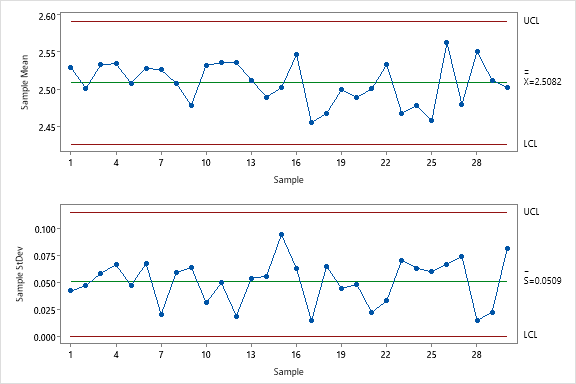
\includegraphics[width=0.75\textwidth]{Xbar_S_Paper.png}
\end{figure}


\item Una empresa que fabrica tarjetas de circuitos impresos desea evaluar si la implementaci\'on de un nuevo sistema de ensamblaje ha reducido el n\'umero de disconformidades. Se tomaron 50 mediciones, antes y después del cambio, para analizar los efectos.
\begin{center}
\begin{tabular}{|l|c|c|}
\hline
 & Antes & Después \\ 
\hline
Media muestral & 3.60 & 2.37 \\ 
\hline
Desviaci'on est'andar muestral & 1.09 & 1.62 \\ 
\hline
\end{tabular}
\end{center}
\begin{enumerate}
\item (15 pts) Calcula un intervalo de confianza de 90\% para el número medio de disconformidades antes del cambio.
\item (15 pts) Calcula un intervalo de confianza de 90\% para la estimar la diferencia en el número medio de disconformidades antes y después del cambio. ¿Qu\'e puedes concluir con este resultado?
\end{enumerate}


\end{enumerate}
  
\newpage



\begin{center}
{\large Instituto Tecnol\'{o}gico y de Estudios Superiores de Monterrey \\
An\'alisis Estad\'stico de Datos } \\
Examen Argumentativo (Papel)
\end{center}

Nombre: \underline{\hspace*{.2in}}
Raúl Hernández
\underline{\hspace*{.2in}} \quad Matr\'icula:\underline{\hspace*{.2in}}
A00000010
\underline{\hspace*{.2in}} \\

{\bf Instrucciones:} Lee con cuidado cada problema y escribe la soluci\'on
en tu hoja de respuesta. Incluye tu procedimiento que muestre c\'omo obtienes tu respuesta.  Respeta el c\'odigo de \'etica del curso y del Tecnol\'ogico de Monterrey y responde los ejercicios de manera individual sin ayuda externa o no autorizada.

\begin{enumerate}

\item Una empresa que fabrica l\'aminas de aluminio para la industria aeron\'autica necesita asegurar que el espesor de sus l\'aminas cumple con las especificaciones de $2.5 \pm 0.1$ mm. Se ha implementado una nueva maquinaria y se desea monitorear el espesor de las l\'aminas. Para ello, se han tomado muestras de tama\~no 4 cada hora y se gener\'o el diagrama que se muestra abajo.
\begin{enumerate}
\item (5 pts) Calcula la media y variabilidad del proceso (dentro de grupos).
\item (10 pts) Calcula los l\'imites de control para el espesor de las láminas.
\item (10 pts) Calcula el porcentaje de l\'aminas que cumplen con las especificaciones. Use los valores del inciso a) para calcular este porcentaje.
\end{enumerate}
\begin{figure}[h!]
\centering
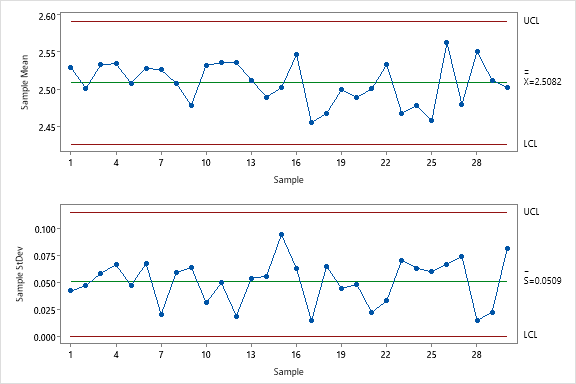
\includegraphics[width=0.75\textwidth]{Xbar_S_Paper.png}
\end{figure}


\item Una empresa que fabrica tarjetas de circuitos impresos desea evaluar si la implementaci\'on de un nuevo sistema de ensamblaje ha reducido el n\'umero de disconformidades. Se tomaron 50 mediciones, antes y después del cambio, para analizar los efectos.
\begin{center}
\begin{tabular}{|l|c|c|}
\hline
 & Antes & Después \\ 
\hline
Media muestral & 3.60 & 2.37 \\ 
\hline
Desviaci'on est'andar muestral & 1.09 & 1.62 \\ 
\hline
\end{tabular}
\end{center}
\begin{enumerate}
\item (15 pts) Calcula un intervalo de confianza de 90\% para el número medio de disconformidades antes del cambio.
\item (15 pts) Calcula un intervalo de confianza de 90\% para la estimar la diferencia en el número medio de disconformidades antes y después del cambio. ¿Qu\'e puedes concluir con este resultado?
\end{enumerate}


\end{enumerate}
  
\newpage



\begin{center}
{\large Instituto Tecnol\'{o}gico y de Estudios Superiores de Monterrey \\
An\'alisis Estad\'stico de Datos } \\
Examen Argumentativo (Papel)
\end{center}

Nombre: \underline{\hspace*{.2in}}
Alejandra Vega
\underline{\hspace*{.2in}} \quad Matr\'icula:\underline{\hspace*{.2in}}
A00000011
\underline{\hspace*{.2in}} \\

{\bf Instrucciones:} Lee con cuidado cada problema y escribe la soluci\'on
en tu hoja de respuesta. Incluye tu procedimiento que muestre c\'omo obtienes tu respuesta.  Respeta el c\'odigo de \'etica del curso y del Tecnol\'ogico de Monterrey y responde los ejercicios de manera individual sin ayuda externa o no autorizada.

\begin{enumerate}

\item Una empresa que fabrica l\'aminas de aluminio para la industria aeron\'autica necesita asegurar que el espesor de sus l\'aminas cumple con las especificaciones de $2.5 \pm 0.1$ mm. Se ha implementado una nueva maquinaria y se desea monitorear el espesor de las l\'aminas. Para ello, se han tomado muestras de tama\~no 4 cada hora y se gener\'o el diagrama que se muestra abajo.
\begin{enumerate}
\item (5 pts) Calcula la media y variabilidad del proceso (dentro de grupos).
\item (10 pts) Calcula los l\'imites de control para la {\bf variabilidad} del espesor de las láminas.
\item (10 pts) Calcula el porcentaje de l\'aminas que tienen un espesor mayor a 2.6 mm. Use los valores del inciso a) para calcular este porcentaje.
\end{enumerate}
\begin{figure}[h!]
\centering
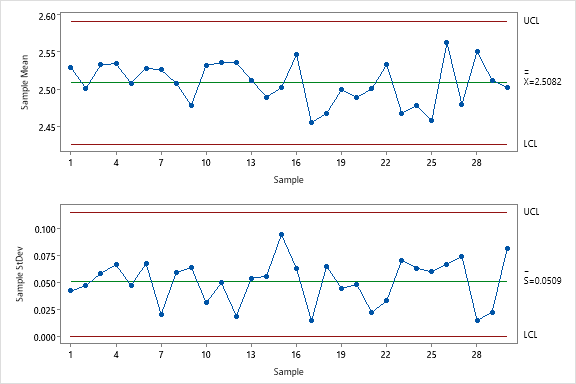
\includegraphics[width=0.75\textwidth]{Xbar_S_Paper.png}
\end{figure}


\item Una empresa que fabrica tarjetas de circuitos impresos desea evaluar si la implementaci\'on de un nuevo sistema de ensamblaje ha reducido el n\'umero de disconformidades. Se tomaron 50 mediciones, antes y después del cambio, para analizar los efectos.
\begin{center}
\begin{tabular}{|l|c|c|}
\hline
 & Antes & Después \\ 
\hline
Media muestral & 3.60 & 2.37 \\ 
\hline
Desviaci'on est'andar muestral & 1.09 & 1.62 \\ 
\hline
\end{tabular}
\end{center}
\begin{enumerate}
\item (15 pts) Calcula un intervalo de confianza de 90\% para el número medio de disconformidades antes del cambio.
\item (15 pts) ¿Existe suficiente evidencia para concluir que el número medio de disconformidades ha disminuido despu\'es del cambio? Usa un nivel de significancia de 0.05.
\end{enumerate}


\end{enumerate}
  
\newpage



\begin{center}
{\large Instituto Tecnol\'{o}gico y de Estudios Superiores de Monterrey \\
An\'alisis Estad\'stico de Datos } \\
Examen Argumentativo (Papel)
\end{center}

Nombre: \underline{\hspace*{.2in}}
César Morales
\underline{\hspace*{.2in}} \quad Matr\'icula:\underline{\hspace*{.2in}}
A00000012
\underline{\hspace*{.2in}} \\

{\bf Instrucciones:} Lee con cuidado cada problema y escribe la soluci\'on
en tu hoja de respuesta. Incluye tu procedimiento que muestre c\'omo obtienes tu respuesta.  Respeta el c\'odigo de \'etica del curso y del Tecnol\'ogico de Monterrey y responde los ejercicios de manera individual sin ayuda externa o no autorizada.

\begin{enumerate}

\item Una empresa que fabrica l\'aminas de aluminio para la industria aeron\'autica necesita asegurar que el espesor de sus l\'aminas cumple con las especificaciones de $2.5 \pm 0.1$ mm. Se ha implementado una nueva maquinaria y se desea monitorear el espesor de las l\'aminas. Para ello, se han tomado muestras de tama\~no 5 cada hora y se gener\'o el diagrama que se muestra abajo.
\begin{enumerate}
\item (5 pts) Calcula la media y variabilidad del proceso (dentro de grupos).
\item (10 pts) Calcula los l\'imites de control para la {\bf variabilidad} del espesor de las láminas.
\item (10 pts) Calcula el porcentaje de l\'aminas que tienen un espesor menor a 2.4 mm. Use los valores del inciso a) para calcular este porcentaje.
\end{enumerate}
\begin{figure}[h!]
\centering
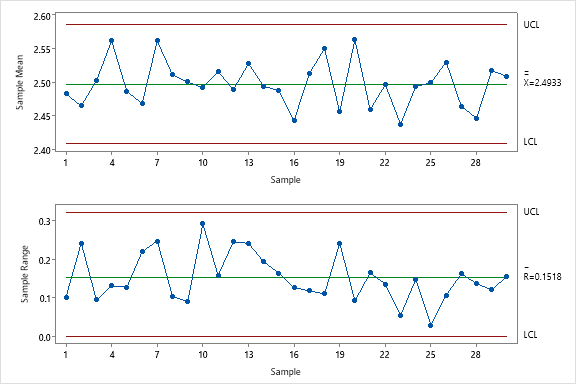
\includegraphics[width=0.75\textwidth]{Xbar_R_Paper.png}
\end{figure}


\item Una empresa que fabrica tarjetas de circuitos impresos desea evaluar si la implementaci\'on de un nuevo sistema de ensamblaje ha reducido el n\'umero de disconformidades. Se tomaron 50 mediciones, antes y después del cambio, para analizar los efectos.
\begin{center}
\begin{tabular}{|l|c|c|}
\hline
 & Antes & Después \\ 
\hline
Media muestral & 3.60 & 2.37 \\ 
\hline
Desviaci'on est'andar muestral & 1.09 & 1.62 \\ 
\hline
\end{tabular}
\end{center}
\begin{enumerate}
\item (15 pts) Calcula un intervalo de confianza de 90\% para el número medio de disconformidades antes del cambio.
\item (15 pts) ¿Existe suficiente evidencia para concluir que el número medio de disconformidades ha disminuido despu\'es del cambio? Usa un nivel de significancia de 0.05.
\end{enumerate}


\end{enumerate}
  
\newpage



\begin{center}
{\large Instituto Tecnol\'{o}gico y de Estudios Superiores de Monterrey \\
An\'alisis Estad\'stico de Datos } \\
Examen Argumentativo (Papel)
\end{center}

Nombre: \underline{\hspace*{.2in}}
Verónica Acosta
\underline{\hspace*{.2in}} \quad Matr\'icula:\underline{\hspace*{.2in}}
A00000013
\underline{\hspace*{.2in}} \\

{\bf Instrucciones:} Lee con cuidado cada problema y escribe la soluci\'on
en tu hoja de respuesta. Incluye tu procedimiento que muestre c\'omo obtienes tu respuesta.  Respeta el c\'odigo de \'etica del curso y del Tecnol\'ogico de Monterrey y responde los ejercicios de manera individual sin ayuda externa o no autorizada.

\begin{enumerate}

\item En una l\'inea de producci\'on de ejes para motores, el di\'ametro es una caracter\'istica crítica para el ensamblaje adecuado. Las especificaciones del di\'ametro son $50 \pm 0.5$ mm. Se mide el di\'ametro de un eje cada 30 minutos. Despu\'es de 15 horas de mediciones, se obtuvo el gr\'afico IMR con un promedio m\'ovil de orden 2 que se muestra abajo.
\begin{enumerate}
\item (5 pts) Calcula la media y variabilidad del proceso (dentro de grupos).
\item (10 pts) Calcula los l\'imites de control para el di\'ametro del eje.
\item (10 pts) Calcula el porcentaje de ejes que no cumplen con las especificaciones. Use los valores del inciso a) para calcular este porcentaje.
\end{enumerate}
\begin{figure}[h!]
\centering
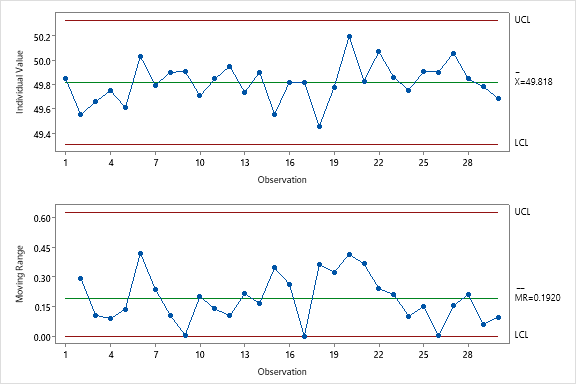
\includegraphics[width=0.75\textwidth]{IMR_Paper.png}
\end{figure}


\item Una empresa que fabrica tarjetas de circuitos impresos desea evaluar si la implementaci\'on de un nuevo sistema de ensamblaje ha reducido el n\'umero de disconformidades. Se tomaron 50 mediciones, antes y después del cambio, para analizar los efectos.
\begin{center}
\begin{tabular}{|l|c|c|}
\hline
 & Antes & Después \\ 
\hline
Media muestral & 3.60 & 2.37 \\ 
\hline
Desviaci'on est'andar muestral & 1.09 & 1.62 \\ 
\hline
\end{tabular}
\end{center}
\begin{enumerate}
\item (15 pts) Calcula un intervalo de confianza de 90\% para el número medio de disconformidades antes del cambio.
\item (15 pts) ¿Existe suficiente evidencia para concluir que el número medio de disconformidades ha disminuido despu\'es del cambio? Usa un nivel de significancia de 0.05.
\end{enumerate}


\end{enumerate}
  
\newpage



\begin{center}
{\large Instituto Tecnol\'{o}gico y de Estudios Superiores de Monterrey \\
An\'alisis Estad\'stico de Datos } \\
Examen Argumentativo (Papel)
\end{center}

Nombre: \underline{\hspace*{.2in}}
Jorge Castillo
\underline{\hspace*{.2in}} \quad Matr\'icula:\underline{\hspace*{.2in}}
A00000014
\underline{\hspace*{.2in}} \\

{\bf Instrucciones:} Lee con cuidado cada problema y escribe la soluci\'on
en tu hoja de respuesta. Incluye tu procedimiento que muestre c\'omo obtienes tu respuesta.  Respeta el c\'odigo de \'etica del curso y del Tecnol\'ogico de Monterrey y responde los ejercicios de manera individual sin ayuda externa o no autorizada.

\begin{enumerate}

\item Una empresa que fabrica l\'aminas de aluminio para la industria aeron\'autica necesita asegurar que el espesor de sus l\'aminas cumple con las especificaciones de $2.5 \pm 0.1$ mm. Se ha implementado una nueva maquinaria y se desea monitorear el espesor de las l\'aminas. Para ello, se han tomado muestras de tama\~no 5 cada hora y se gener\'o el diagrama que se muestra abajo.
\begin{enumerate}
\item (5 pts) Calcula la media y variabilidad del proceso (dentro de grupos).
\item (10 pts) Calcula los l\'imites de control para el espesor de las láminas.
\item (10 pts) Calcula el porcentaje de l\'aminas que no cumplen con las especificaciones. Use los valores del inciso a) para calcular este porcentaje.
\end{enumerate}
\begin{figure}[h!]
\centering
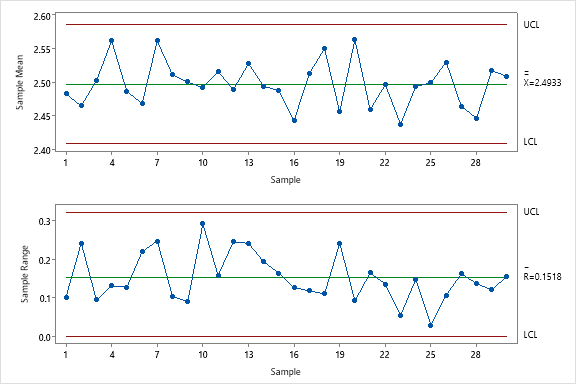
\includegraphics[width=0.75\textwidth]{Xbar_R_Paper.png}
\end{figure}


\item Una empresa que fabrica tarjetas de circuitos impresos desea evaluar si la implementaci\'on de un nuevo sistema de ensamblaje ha reducido el n\'umero de disconformidades. Se tomaron 50 mediciones, antes y después del cambio, para analizar los efectos.
\begin{center}
\begin{tabular}{|l|c|c|}
\hline
 & Antes & Después \\ 
\hline
Media muestral & 3.60 & 2.37 \\ 
\hline
Desviaci'on est'andar muestral & 1.09 & 1.62 \\ 
\hline
\end{tabular}
\end{center}
\begin{enumerate}
\item (15 pts) Calcula un intervalo de confianza de 90\% para el número medio de disconformidades antes del cambio.
\item (15 pts) Calcula un intervalo de confianza de 90\% para la estimar la diferencia en el número medio de disconformidades antes y después del cambio. ¿Qu\'e puedes concluir con este resultado?
\end{enumerate}


\end{enumerate}
  
\newpage



\begin{center}
{\large Instituto Tecnol\'{o}gico y de Estudios Superiores de Monterrey \\
An\'alisis Estad\'stico de Datos } \\
Examen Argumentativo (Papel)
\end{center}

Nombre: \underline{\hspace*{.2in}}
Diana Navarro
\underline{\hspace*{.2in}} \quad Matr\'icula:\underline{\hspace*{.2in}}
A00000015
\underline{\hspace*{.2in}} \\

{\bf Instrucciones:} Lee con cuidado cada problema y escribe la soluci\'on
en tu hoja de respuesta. Incluye tu procedimiento que muestre c\'omo obtienes tu respuesta.  Respeta el c\'odigo de \'etica del curso y del Tecnol\'ogico de Monterrey y responde los ejercicios de manera individual sin ayuda externa o no autorizada.

\begin{enumerate}

\item Una empresa que fabrica l\'aminas de aluminio para la industria aeron\'autica necesita asegurar que el espesor de sus l\'aminas cumple con las especificaciones de $2.5 \pm 0.1$ mm. Se ha implementado una nueva maquinaria y se desea monitorear el espesor de las l\'aminas. Para ello, se han tomado muestras de tama\~no 4 cada hora y se gener\'o el diagrama que se muestra abajo.
\begin{enumerate}
\item (5 pts) Calcula la media y variabilidad del proceso (dentro de grupos).
\item (10 pts) Calcula los l\'imites de control para el espesor de las láminas.
\item (10 pts) Calcula el porcentaje de l\'aminas que cumplen con las especificaciones. Use los valores del inciso a) para calcular este porcentaje.
\end{enumerate}
\begin{figure}[h!]
\centering
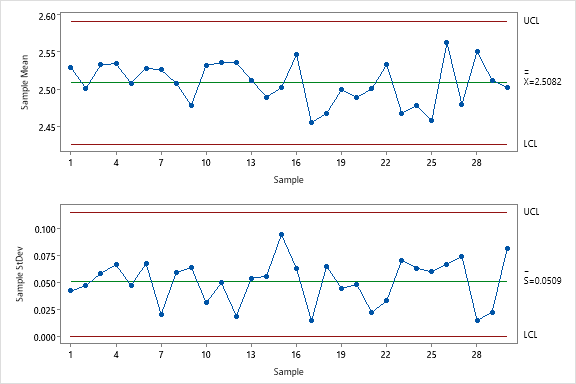
\includegraphics[width=0.75\textwidth]{Xbar_S_Paper.png}
\end{figure}


\item Una empresa que fabrica tarjetas de circuitos impresos desea evaluar si la implementaci\'on de un nuevo sistema de ensamblaje ha reducido el n\'umero de disconformidades. Se tomaron 50 mediciones, antes y después del cambio, para analizar los efectos.
\begin{center}
\begin{tabular}{|l|c|c|}
\hline
 & Antes & Después \\ 
\hline
Media muestral & 3.60 & 2.37 \\ 
\hline
Desviaci'on est'andar muestral & 1.09 & 1.62 \\ 
\hline
\end{tabular}
\end{center}
\begin{enumerate}
\item (15 pts) Calcula un intervalo de confianza de 90\% para el número medio de disconformidades antes del cambio.
\item (15 pts) ¿Existe suficiente evidencia para concluir que el número medio de disconformidades ha disminuido despu\'es del cambio? Usa un nivel de significancia de 0.05.
\end{enumerate}


\end{enumerate}
  
\newpage



\begin{center}
{\large Instituto Tecnol\'{o}gico y de Estudios Superiores de Monterrey \\
An\'alisis Estad\'stico de Datos } \\
Examen Argumentativo (Papel)
\end{center}

Nombre: \underline{\hspace*{.2in}}
Manuel Cota
\underline{\hspace*{.2in}} \quad Matr\'icula:\underline{\hspace*{.2in}}
A00000016
\underline{\hspace*{.2in}} \\

{\bf Instrucciones:} Lee con cuidado cada problema y escribe la soluci\'on
en tu hoja de respuesta. Incluye tu procedimiento que muestre c\'omo obtienes tu respuesta.  Respeta el c\'odigo de \'etica del curso y del Tecnol\'ogico de Monterrey y responde los ejercicios de manera individual sin ayuda externa o no autorizada.

\begin{enumerate}

\item Una empresa que fabrica l\'aminas de aluminio para la industria aeron\'autica necesita asegurar que el espesor de sus l\'aminas cumple con las especificaciones de $2.5 \pm 0.1$ mm. Se ha implementado una nueva maquinaria y se desea monitorear el espesor de las l\'aminas. Para ello, se han tomado muestras de tama\~no 4 cada hora y se gener\'o el diagrama que se muestra abajo.
\begin{enumerate}
\item (5 pts) Calcula la media y variabilidad del proceso (dentro de grupos).
\item (10 pts) Calcula los l\'imites de control para el espesor de las láminas.
\item (10 pts) Calcula el porcentaje de l\'aminas que cumplen con las especificaciones. Use los valores del inciso a) para calcular este porcentaje.
\end{enumerate}
\begin{figure}[h!]
\centering
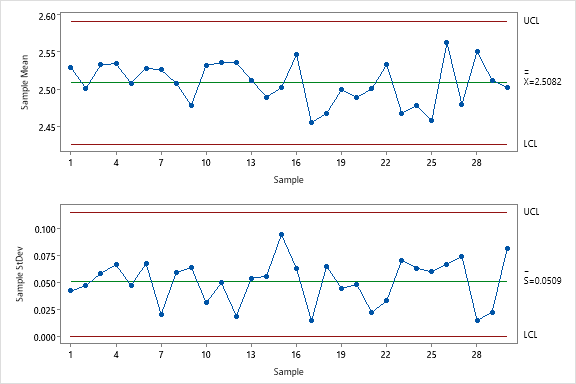
\includegraphics[width=0.75\textwidth]{Xbar_S_Paper.png}
\end{figure}


\item Una empresa que fabrica tarjetas de circuitos impresos desea evaluar si la implementaci\'on de un nuevo sistema de ensamblaje ha reducido el n\'umero de disconformidades. Se tomaron 50 mediciones, antes y después del cambio, para analizar los efectos.
\begin{center}
\begin{tabular}{|l|c|c|}
\hline
 & Antes & Después \\ 
\hline
Media muestral & 3.60 & 2.37 \\ 
\hline
Desviaci'on est'andar muestral & 1.09 & 1.62 \\ 
\hline
\end{tabular}
\end{center}
\begin{enumerate}
\item (15 pts) Calcula un intervalo de confianza de 90\% para el número medio de disconformidades antes del cambio.
\item (15 pts) Calcula un intervalo de confianza de 90\% para la estimar la diferencia en el número medio de disconformidades antes y después del cambio. ¿Qu\'e puedes concluir con este resultado?
\end{enumerate}


\end{enumerate}
  
\newpage



\begin{center}
{\large Instituto Tecnol\'{o}gico y de Estudios Superiores de Monterrey \\
An\'alisis Estad\'stico de Datos } \\
Examen Argumentativo (Papel)
\end{center}

Nombre: \underline{\hspace*{.2in}}
Sofía Delgado
\underline{\hspace*{.2in}} \quad Matr\'icula:\underline{\hspace*{.2in}}
A00000017
\underline{\hspace*{.2in}} \\

{\bf Instrucciones:} Lee con cuidado cada problema y escribe la soluci\'on
en tu hoja de respuesta. Incluye tu procedimiento que muestre c\'omo obtienes tu respuesta.  Respeta el c\'odigo de \'etica del curso y del Tecnol\'ogico de Monterrey y responde los ejercicios de manera individual sin ayuda externa o no autorizada.

\begin{enumerate}

\item Una empresa que fabrica l\'aminas de aluminio para la industria aeron\'autica necesita asegurar que el espesor de sus l\'aminas cumple con las especificaciones de $2.5 \pm 0.1$ mm. Se ha implementado una nueva maquinaria y se desea monitorear el espesor de las l\'aminas. Para ello, se han tomado muestras de tama\~no 5 cada hora y se gener\'o el diagrama que se muestra abajo.
\begin{enumerate}
\item (5 pts) Calcula la media y variabilidad del proceso (dentro de grupos).
\item (10 pts) Calcula los l\'imites de control para la {\bf variabilidad} del espesor de las láminas.
\item (10 pts) Calcula el porcentaje de l\'aminas que tienen un espesor menor a 2.4 mm. Use los valores del inciso a) para calcular este porcentaje.
\end{enumerate}
\begin{figure}[h!]
\centering
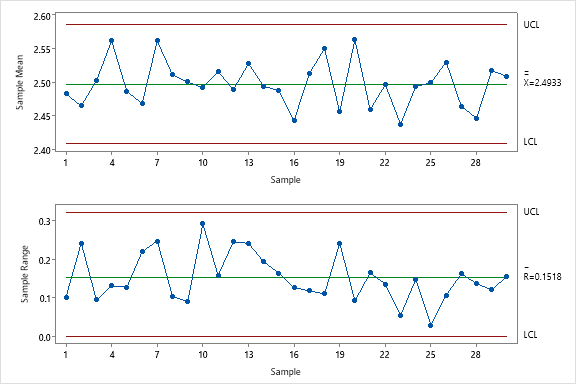
\includegraphics[width=0.75\textwidth]{Xbar_R_Paper.png}
\end{figure}


\item Una empresa que fabrica tarjetas de circuitos impresos desea evaluar si la implementaci\'on de un nuevo sistema de ensamblaje ha reducido el n\'umero de disconformidades. Se tomaron 50 mediciones, antes y después del cambio, para analizar los efectos.
\begin{center}
\begin{tabular}{|l|c|c|}
\hline
 & Antes & Después \\ 
\hline
Media muestral & 3.60 & 2.37 \\ 
\hline
Desviaci'on est'andar muestral & 1.09 & 1.62 \\ 
\hline
\end{tabular}
\end{center}
\begin{enumerate}
\item (15 pts) Calcula un intervalo de confianza de 90\% para el número medio de disconformidades antes del cambio.
\item (15 pts) Calcula un intervalo de confianza de 90\% para la estimar la diferencia en el número medio de disconformidades antes y después del cambio. ¿Qu\'e puedes concluir con este resultado?
\end{enumerate}


\end{enumerate}
  
\newpage



\begin{center}
{\large Instituto Tecnol\'{o}gico y de Estudios Superiores de Monterrey \\
An\'alisis Estad\'stico de Datos } \\
Examen Argumentativo (Papel)
\end{center}

Nombre: \underline{\hspace*{.2in}}
Roberto Beltrán
\underline{\hspace*{.2in}} \quad Matr\'icula:\underline{\hspace*{.2in}}
A00000018
\underline{\hspace*{.2in}} \\

{\bf Instrucciones:} Lee con cuidado cada problema y escribe la soluci\'on
en tu hoja de respuesta. Incluye tu procedimiento que muestre c\'omo obtienes tu respuesta.  Respeta el c\'odigo de \'etica del curso y del Tecnol\'ogico de Monterrey y responde los ejercicios de manera individual sin ayuda externa o no autorizada.

\begin{enumerate}

\item Una empresa que fabrica l\'aminas de aluminio para la industria aeron\'autica necesita asegurar que el espesor de sus l\'aminas cumple con las especificaciones de $2.5 \pm 0.1$ mm. Se ha implementado una nueva maquinaria y se desea monitorear el espesor de las l\'aminas. Para ello, se han tomado muestras de tama\~no 4 cada hora y se gener\'o el diagrama que se muestra abajo.
\begin{enumerate}
\item (5 pts) Calcula la media y variabilidad del proceso (dentro de grupos).
\item (10 pts) Calcula los l\'imites de control para el espesor de las láminas.
\item (10 pts) Calcula el porcentaje de l\'aminas que cumplen con las especificaciones. Use los valores del inciso a) para calcular este porcentaje.
\end{enumerate}
\begin{figure}[h!]
\centering
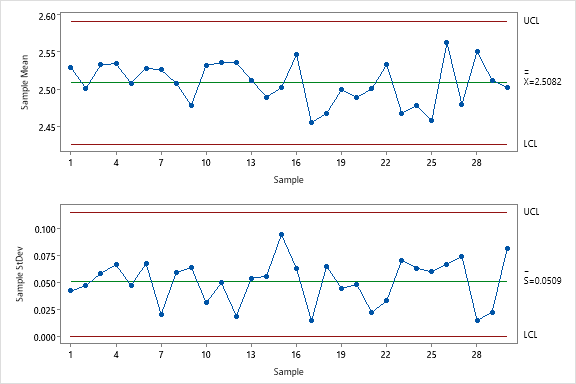
\includegraphics[width=0.75\textwidth]{Xbar_S_Paper.png}
\end{figure}


\item Una empresa que fabrica tarjetas de circuitos impresos desea evaluar si la implementaci\'on de un nuevo sistema de ensamblaje ha reducido el n\'umero de disconformidades. Se tomaron 50 mediciones, antes y después del cambio, para analizar los efectos.
\begin{center}
\begin{tabular}{|l|c|c|}
\hline
 & Antes & Después \\ 
\hline
Media muestral & 3.60 & 2.37 \\ 
\hline
Desviaci'on est'andar muestral & 1.09 & 1.62 \\ 
\hline
\end{tabular}
\end{center}
\begin{enumerate}
\item (15 pts) Calcula un intervalo de confianza de 90\% para el número medio de disconformidades antes del cambio.
\item (15 pts) ¿Existe suficiente evidencia para concluir que el número medio de disconformidades ha disminuido despu\'es del cambio? Usa un nivel de significancia de 0.05.
\end{enumerate}


\end{enumerate}
  
\newpage



\begin{center}
{\large Instituto Tecnol\'{o}gico y de Estudios Superiores de Monterrey \\
An\'alisis Estad\'stico de Datos } \\
Examen Argumentativo (Papel)
\end{center}

Nombre: \underline{\hspace*{.2in}}
Mariana Ibarra
\underline{\hspace*{.2in}} \quad Matr\'icula:\underline{\hspace*{.2in}}
A00000019
\underline{\hspace*{.2in}} \\

{\bf Instrucciones:} Lee con cuidado cada problema y escribe la soluci\'on
en tu hoja de respuesta. Incluye tu procedimiento que muestre c\'omo obtienes tu respuesta.  Respeta el c\'odigo de \'etica del curso y del Tecnol\'ogico de Monterrey y responde los ejercicios de manera individual sin ayuda externa o no autorizada.

\begin{enumerate}

\item Una empresa que fabrica l\'aminas de aluminio para la industria aeron\'autica necesita asegurar que el espesor de sus l\'aminas cumple con las especificaciones de $2.5 \pm 0.1$ mm. Se ha implementado una nueva maquinaria y se desea monitorear el espesor de las l\'aminas. Para ello, se han tomado muestras de tama\~no 5 cada hora y se gener\'o el diagrama que se muestra abajo.
\begin{enumerate}
\item (5 pts) Calcula la media y variabilidad del proceso (dentro de grupos).
\item (10 pts) Calcula los l\'imites de control para la {\bf variabilidad} del espesor de las láminas.
\item (10 pts) Calcula el porcentaje de l\'aminas que tienen un espesor menor a 2.4 mm. Use los valores del inciso a) para calcular este porcentaje.
\end{enumerate}
\begin{figure}[h!]
\centering
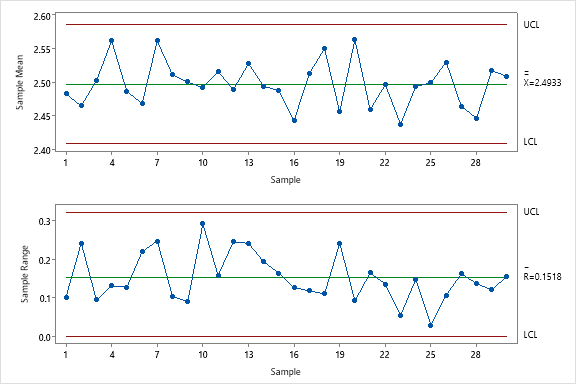
\includegraphics[width=0.75\textwidth]{Xbar_R_Paper.png}
\end{figure}


\item Una empresa que fabrica tarjetas de circuitos impresos desea evaluar si la implementaci\'on de un nuevo sistema de ensamblaje ha reducido el n\'umero de disconformidades. Se tomaron 50 mediciones, antes y después del cambio, para analizar los efectos.
\begin{center}
\begin{tabular}{|l|c|c|}
\hline
 & Antes & Después \\ 
\hline
Media muestral & 3.60 & 2.37 \\ 
\hline
Desviaci'on est'andar muestral & 1.09 & 1.62 \\ 
\hline
\end{tabular}
\end{center}
\begin{enumerate}
\item (15 pts) Calcula un intervalo de confianza de 90\% para el número medio de disconformidades antes del cambio.
\item (15 pts) ¿Existe suficiente evidencia para concluir que el número medio de disconformidades ha disminuido despu\'es del cambio? Usa un nivel de significancia de 0.05.
\end{enumerate}


\end{enumerate}
  
\newpage



\begin{center}
{\large Instituto Tecnol\'{o}gico y de Estudios Superiores de Monterrey \\
An\'alisis Estad\'stico de Datos } \\
Examen Argumentativo (Papel)
\end{center}

Nombre: \underline{\hspace*{.2in}}
Ernesto Valdez
\underline{\hspace*{.2in}} \quad Matr\'icula:\underline{\hspace*{.2in}}
A00000020
\underline{\hspace*{.2in}} \\

{\bf Instrucciones:} Lee con cuidado cada problema y escribe la soluci\'on
en tu hoja de respuesta. Incluye tu procedimiento que muestre c\'omo obtienes tu respuesta.  Respeta el c\'odigo de \'etica del curso y del Tecnol\'ogico de Monterrey y responde los ejercicios de manera individual sin ayuda externa o no autorizada.

\begin{enumerate}

\item Una empresa que fabrica l\'aminas de aluminio para la industria aeron\'autica necesita asegurar que el espesor de sus l\'aminas cumple con las especificaciones de $2.5 \pm 0.1$ mm. Se ha implementado una nueva maquinaria y se desea monitorear el espesor de las l\'aminas. Para ello, se han tomado muestras de tama\~no 5 cada hora y se gener\'o el diagrama que se muestra abajo.
\begin{enumerate}
\item (5 pts) Calcula la media y variabilidad del proceso (dentro de grupos).
\item (10 pts) Calcula los l\'imites de control para el espesor de las láminas.
\item (10 pts) Calcula el porcentaje de l\'aminas que no cumplen con las especificaciones. Use los valores del inciso a) para calcular este porcentaje.
\end{enumerate}
\begin{figure}[h!]
\centering
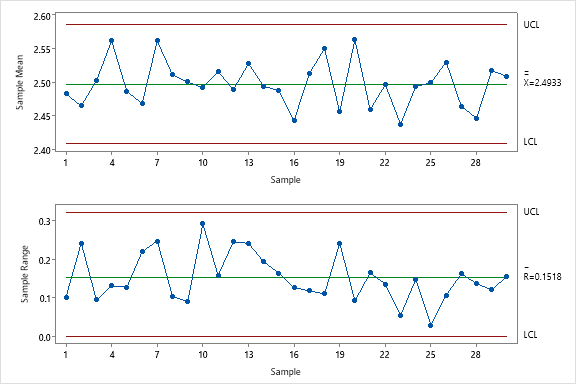
\includegraphics[width=0.75\textwidth]{Xbar_R_Paper.png}
\end{figure}


\item Una empresa que fabrica tarjetas de circuitos impresos desea evaluar si la implementaci\'on de un nuevo sistema de ensamblaje ha reducido el n\'umero de disconformidades. Se tomaron 50 mediciones, antes y después del cambio, para analizar los efectos.
\begin{center}
\begin{tabular}{|l|c|c|}
\hline
 & Antes & Después \\ 
\hline
Media muestral & 3.60 & 2.37 \\ 
\hline
Desviaci'on est'andar muestral & 1.09 & 1.62 \\ 
\hline
\end{tabular}
\end{center}
\begin{enumerate}
\item (15 pts) Calcula un intervalo de confianza de 90\% para el número medio de disconformidades antes del cambio.
\item (15 pts) ¿Existe suficiente evidencia para concluir que el número medio de disconformidades ha disminuido despu\'es del cambio? Usa un nivel de significancia de 0.05.
\end{enumerate}


\end{enumerate}
  
\newpage



\begin{center}
{\large Instituto Tecnol\'{o}gico y de Estudios Superiores de Monterrey \\
An\'alisis Estad\'stico de Datos } \\
Examen Argumentativo (Papel)
\end{center}

Nombre: \underline{\hspace*{.2in}}
Paulina Espinoza
\underline{\hspace*{.2in}} \quad Matr\'icula:\underline{\hspace*{.2in}}
A00000021
\underline{\hspace*{.2in}} \\

{\bf Instrucciones:} Lee con cuidado cada problema y escribe la soluci\'on
en tu hoja de respuesta. Incluye tu procedimiento que muestre c\'omo obtienes tu respuesta.  Respeta el c\'odigo de \'etica del curso y del Tecnol\'ogico de Monterrey y responde los ejercicios de manera individual sin ayuda externa o no autorizada.

\begin{enumerate}

\item Una empresa que fabrica l\'aminas de aluminio para la industria aeron\'autica necesita asegurar que el espesor de sus l\'aminas cumple con las especificaciones de $2.5 \pm 0.1$ mm. Se ha implementado una nueva maquinaria y se desea monitorear el espesor de las l\'aminas. Para ello, se han tomado muestras de tama\~no 4 cada hora y se gener\'o el diagrama que se muestra abajo.
\begin{enumerate}
\item (5 pts) Calcula la media y variabilidad del proceso (dentro de grupos).
\item (10 pts) Calcula los l\'imites de control para el espesor de las láminas.
\item (10 pts) Calcula el porcentaje de l\'aminas que cumplen con las especificaciones. Use los valores del inciso a) para calcular este porcentaje.
\end{enumerate}
\begin{figure}[h!]
\centering
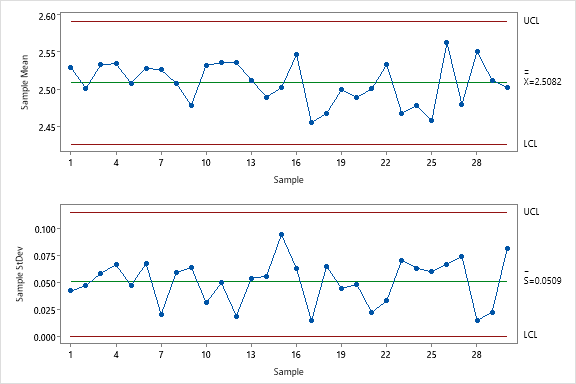
\includegraphics[width=0.75\textwidth]{Xbar_S_Paper.png}
\end{figure}


\item Una empresa que fabrica tarjetas de circuitos impresos desea evaluar si la implementaci\'on de un nuevo sistema de ensamblaje ha reducido el n\'umero de disconformidades. Se tomaron 50 mediciones, antes y después del cambio, para analizar los efectos.
\begin{center}
\begin{tabular}{|l|c|c|}
\hline
 & Antes & Después \\ 
\hline
Media muestral & 3.60 & 2.37 \\ 
\hline
Desviaci'on est'andar muestral & 1.09 & 1.62 \\ 
\hline
\end{tabular}
\end{center}
\begin{enumerate}
\item (15 pts) Calcula un intervalo de confianza de 90\% para el número medio de disconformidades antes del cambio.
\item (15 pts) Calcula un intervalo de confianza de 90\% para la estimar la diferencia en el número medio de disconformidades antes y después del cambio. ¿Qu\'e puedes concluir con este resultado?
\end{enumerate}


\end{enumerate}
  
\newpage



\begin{center}
{\large Instituto Tecnol\'{o}gico y de Estudios Superiores de Monterrey \\
An\'alisis Estad\'stico de Datos } \\
Examen Argumentativo (Papel)
\end{center}

Nombre: \underline{\hspace*{.2in}}
Sergio Medina
\underline{\hspace*{.2in}} \quad Matr\'icula:\underline{\hspace*{.2in}}
A00000022
\underline{\hspace*{.2in}} \\

{\bf Instrucciones:} Lee con cuidado cada problema y escribe la soluci\'on
en tu hoja de respuesta. Incluye tu procedimiento que muestre c\'omo obtienes tu respuesta.  Respeta el c\'odigo de \'etica del curso y del Tecnol\'ogico de Monterrey y responde los ejercicios de manera individual sin ayuda externa o no autorizada.

\begin{enumerate}

\item Una empresa que fabrica l\'aminas de aluminio para la industria aeron\'autica necesita asegurar que el espesor de sus l\'aminas cumple con las especificaciones de $2.5 \pm 0.1$ mm. Se ha implementado una nueva maquinaria y se desea monitorear el espesor de las l\'aminas. Para ello, se han tomado muestras de tama\~no 4 cada hora y se gener\'o el diagrama que se muestra abajo.
\begin{enumerate}
\item (5 pts) Calcula la media y variabilidad del proceso (dentro de grupos).
\item (10 pts) Calcula los l\'imites de control para la {\bf variabilidad} del espesor de las láminas.
\item (10 pts) Calcula el porcentaje de l\'aminas que tienen un espesor mayor a 2.6 mm. Use los valores del inciso a) para calcular este porcentaje.
\end{enumerate}
\begin{figure}[h!]
\centering
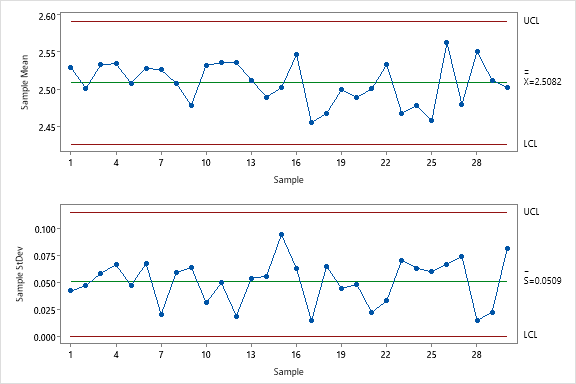
\includegraphics[width=0.75\textwidth]{Xbar_S_Paper.png}
\end{figure}


\item Una empresa que fabrica tarjetas de circuitos impresos desea evaluar si la implementaci\'on de un nuevo sistema de ensamblaje ha reducido el n\'umero de disconformidades. Se tomaron 50 mediciones, antes y después del cambio, para analizar los efectos.
\begin{center}
\begin{tabular}{|l|c|c|}
\hline
 & Antes & Después \\ 
\hline
Media muestral & 3.60 & 2.37 \\ 
\hline
Desviaci'on est'andar muestral & 1.09 & 1.62 \\ 
\hline
\end{tabular}
\end{center}
\begin{enumerate}
\item (15 pts) Calcula un intervalo de confianza de 90\% para el número medio de disconformidades antes del cambio.
\item (15 pts) Calcula un intervalo de confianza de 90\% para la estimar la diferencia en el número medio de disconformidades antes y después del cambio. ¿Qu\'e puedes concluir con este resultado?
\end{enumerate}


\end{enumerate}
  
\newpage



\begin{center}
{\large Instituto Tecnol\'{o}gico y de Estudios Superiores de Monterrey \\
An\'alisis Estad\'stico de Datos } \\
Examen Argumentativo (Papel)
\end{center}

Nombre: \underline{\hspace*{.2in}}
Brenda Aguilar
\underline{\hspace*{.2in}} \quad Matr\'icula:\underline{\hspace*{.2in}}
A00000023
\underline{\hspace*{.2in}} \\

{\bf Instrucciones:} Lee con cuidado cada problema y escribe la soluci\'on
en tu hoja de respuesta. Incluye tu procedimiento que muestre c\'omo obtienes tu respuesta.  Respeta el c\'odigo de \'etica del curso y del Tecnol\'ogico de Monterrey y responde los ejercicios de manera individual sin ayuda externa o no autorizada.

\begin{enumerate}

\item Una empresa que fabrica l\'aminas de aluminio para la industria aeron\'autica necesita asegurar que el espesor de sus l\'aminas cumple con las especificaciones de $2.5 \pm 0.1$ mm. Se ha implementado una nueva maquinaria y se desea monitorear el espesor de las l\'aminas. Para ello, se han tomado muestras de tama\~no 4 cada hora y se gener\'o el diagrama que se muestra abajo.
\begin{enumerate}
\item (5 pts) Calcula la media y variabilidad del proceso (dentro de grupos).
\item (10 pts) Calcula los l\'imites de control para el espesor de las láminas.
\item (10 pts) Calcula el porcentaje de l\'aminas que cumplen con las especificaciones. Use los valores del inciso a) para calcular este porcentaje.
\end{enumerate}
\begin{figure}[h!]
\centering
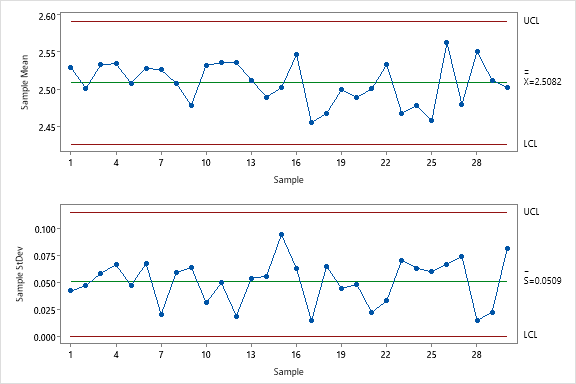
\includegraphics[width=0.75\textwidth]{Xbar_S_Paper.png}
\end{figure}


\item Una empresa que fabrica tarjetas de circuitos impresos desea evaluar si la implementaci\'on de un nuevo sistema de ensamblaje ha reducido el n\'umero de disconformidades. Se tomaron 50 mediciones, antes y después del cambio, para analizar los efectos.
\begin{center}
\begin{tabular}{|l|c|c|}
\hline
 & Antes & Después \\ 
\hline
Media muestral & 3.60 & 2.37 \\ 
\hline
Desviaci'on est'andar muestral & 1.09 & 1.62 \\ 
\hline
\end{tabular}
\end{center}
\begin{enumerate}
\item (15 pts) Calcula un intervalo de confianza de 90\% para el número medio de disconformidades antes del cambio.
\item (15 pts) Calcula un intervalo de confianza de 90\% para la estimar la diferencia en el número medio de disconformidades antes y después del cambio. ¿Qu\'e puedes concluir con este resultado?
\end{enumerate}


\end{enumerate}
  
\newpage



\begin{center}
{\large Instituto Tecnol\'{o}gico y de Estudios Superiores de Monterrey \\
An\'alisis Estad\'stico de Datos } \\
Examen Argumentativo (Papel)
\end{center}

Nombre: \underline{\hspace*{.2in}}
Héctor Fuentes
\underline{\hspace*{.2in}} \quad Matr\'icula:\underline{\hspace*{.2in}}
A00000024
\underline{\hspace*{.2in}} \\

{\bf Instrucciones:} Lee con cuidado cada problema y escribe la soluci\'on
en tu hoja de respuesta. Incluye tu procedimiento que muestre c\'omo obtienes tu respuesta.  Respeta el c\'odigo de \'etica del curso y del Tecnol\'ogico de Monterrey y responde los ejercicios de manera individual sin ayuda externa o no autorizada.

\begin{enumerate}

\item Una empresa que fabrica l\'aminas de aluminio para la industria aeron\'autica necesita asegurar que el espesor de sus l\'aminas cumple con las especificaciones de $2.5 \pm 0.1$ mm. Se ha implementado una nueva maquinaria y se desea monitorear el espesor de las l\'aminas. Para ello, se han tomado muestras de tama\~no 5 cada hora y se gener\'o el diagrama que se muestra abajo.
\begin{enumerate}
\item (5 pts) Calcula la media y variabilidad del proceso (dentro de grupos).
\item (10 pts) Calcula los l\'imites de control para el espesor de las láminas.
\item (10 pts) Calcula el porcentaje de l\'aminas que no cumplen con las especificaciones. Use los valores del inciso a) para calcular este porcentaje.
\end{enumerate}
\begin{figure}[h!]
\centering
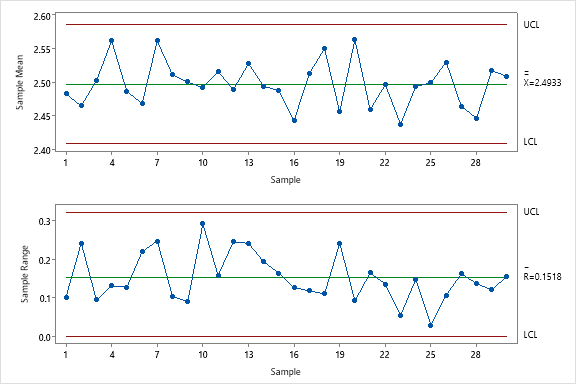
\includegraphics[width=0.75\textwidth]{Xbar_R_Paper.png}
\end{figure}


\item Una empresa que fabrica tarjetas de circuitos impresos desea evaluar si la implementaci\'on de un nuevo sistema de ensamblaje ha reducido el n\'umero de disconformidades. Se tomaron 50 mediciones, antes y después del cambio, para analizar los efectos.
\begin{center}
\begin{tabular}{|l|c|c|}
\hline
 & Antes & Después \\ 
\hline
Media muestral & 3.60 & 2.37 \\ 
\hline
Desviaci'on est'andar muestral & 1.09 & 1.62 \\ 
\hline
\end{tabular}
\end{center}
\begin{enumerate}
\item (15 pts) Calcula un intervalo de confianza de 90\% para el número medio de disconformidades antes del cambio.
\item (15 pts) ¿Existe suficiente evidencia para concluir que el número medio de disconformidades ha disminuido despu\'es del cambio? Usa un nivel de significancia de 0.05.
\end{enumerate}


\end{enumerate}
  
\newpage



\begin{center}
{\large Instituto Tecnol\'{o}gico y de Estudios Superiores de Monterrey \\
An\'alisis Estad\'stico de Datos } \\
Examen Argumentativo (Papel)
\end{center}

Nombre: \underline{\hspace*{.2in}}
Andrea Campos
\underline{\hspace*{.2in}} \quad Matr\'icula:\underline{\hspace*{.2in}}
A00000025
\underline{\hspace*{.2in}} \\

{\bf Instrucciones:} Lee con cuidado cada problema y escribe la soluci\'on
en tu hoja de respuesta. Incluye tu procedimiento que muestre c\'omo obtienes tu respuesta.  Respeta el c\'odigo de \'etica del curso y del Tecnol\'ogico de Monterrey y responde los ejercicios de manera individual sin ayuda externa o no autorizada.

\begin{enumerate}

\item Una empresa que fabrica l\'aminas de aluminio para la industria aeron\'autica necesita asegurar que el espesor de sus l\'aminas cumple con las especificaciones de $2.5 \pm 0.1$ mm. Se ha implementado una nueva maquinaria y se desea monitorear el espesor de las l\'aminas. Para ello, se han tomado muestras de tama\~no 4 cada hora y se gener\'o el diagrama que se muestra abajo.
\begin{enumerate}
\item (5 pts) Calcula la media y variabilidad del proceso (dentro de grupos).
\item (10 pts) Calcula los l\'imites de control para la {\bf variabilidad} del espesor de las láminas.
\item (10 pts) Calcula el porcentaje de l\'aminas que tienen un espesor mayor a 2.6 mm. Use los valores del inciso a) para calcular este porcentaje.
\end{enumerate}
\begin{figure}[h!]
\centering
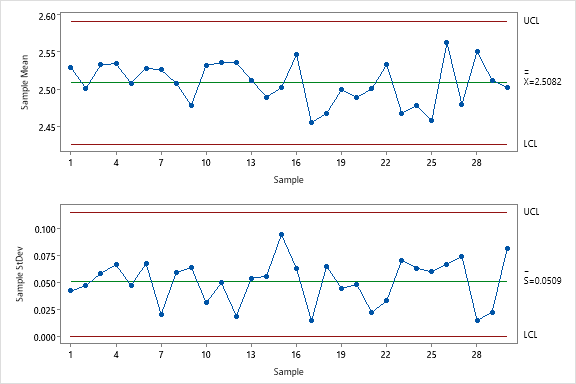
\includegraphics[width=0.75\textwidth]{Xbar_S_Paper.png}
\end{figure}


\item Una empresa que fabrica tarjetas de circuitos impresos desea evaluar si la implementaci\'on de un nuevo sistema de ensamblaje ha reducido el n\'umero de disconformidades. Se tomaron 50 mediciones, antes y después del cambio, para analizar los efectos.
\begin{center}
\begin{tabular}{|l|c|c|}
\hline
 & Antes & Después \\ 
\hline
Media muestral & 3.60 & 2.37 \\ 
\hline
Desviaci'on est'andar muestral & 1.09 & 1.62 \\ 
\hline
\end{tabular}
\end{center}
\begin{enumerate}
\item (15 pts) Calcula un intervalo de confianza de 90\% para el número medio de disconformidades antes del cambio.
\item (15 pts) Calcula un intervalo de confianza de 90\% para la estimar la diferencia en el número medio de disconformidades antes y después del cambio. ¿Qu\'e puedes concluir con este resultado?
\end{enumerate}


\end{enumerate}
  
\newpage



\begin{center}
{\large Instituto Tecnol\'{o}gico y de Estudios Superiores de Monterrey \\
An\'alisis Estad\'stico de Datos } \\
Examen Argumentativo (Papel)
\end{center}

Nombre: \underline{\hspace*{.2in}}
Ricardo Ponce
\underline{\hspace*{.2in}} \quad Matr\'icula:\underline{\hspace*{.2in}}
A00000026
\underline{\hspace*{.2in}} \\

{\bf Instrucciones:} Lee con cuidado cada problema y escribe la soluci\'on
en tu hoja de respuesta. Incluye tu procedimiento que muestre c\'omo obtienes tu respuesta.  Respeta el c\'odigo de \'etica del curso y del Tecnol\'ogico de Monterrey y responde los ejercicios de manera individual sin ayuda externa o no autorizada.

\begin{enumerate}

\item Una empresa que fabrica l\'aminas de aluminio para la industria aeron\'autica necesita asegurar que el espesor de sus l\'aminas cumple con las especificaciones de $2.5 \pm 0.1$ mm. Se ha implementado una nueva maquinaria y se desea monitorear el espesor de las l\'aminas. Para ello, se han tomado muestras de tama\~no 5 cada hora y se gener\'o el diagrama que se muestra abajo.
\begin{enumerate}
\item (5 pts) Calcula la media y variabilidad del proceso (dentro de grupos).
\item (10 pts) Calcula los l\'imites de control para el espesor de las láminas.
\item (10 pts) Calcula el porcentaje de l\'aminas que no cumplen con las especificaciones. Use los valores del inciso a) para calcular este porcentaje.
\end{enumerate}
\begin{figure}[h!]
\centering
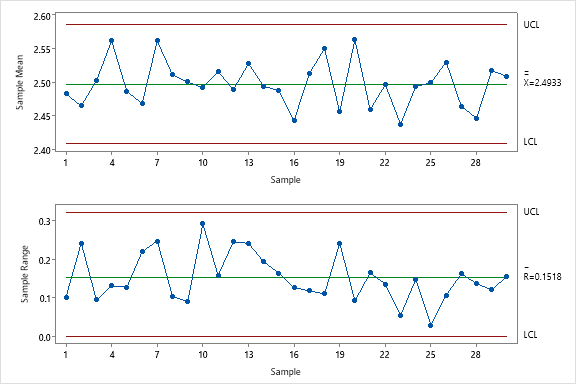
\includegraphics[width=0.75\textwidth]{Xbar_R_Paper.png}
\end{figure}


\item Una empresa que fabrica tarjetas de circuitos impresos desea evaluar si la implementaci\'on de un nuevo sistema de ensamblaje ha reducido el n\'umero de disconformidades. Se tomaron 50 mediciones, antes y después del cambio, para analizar los efectos.
\begin{center}
\begin{tabular}{|l|c|c|}
\hline
 & Antes & Después \\ 
\hline
Media muestral & 3.60 & 2.37 \\ 
\hline
Desviaci'on est'andar muestral & 1.09 & 1.62 \\ 
\hline
\end{tabular}
\end{center}
\begin{enumerate}
\item (15 pts) Calcula un intervalo de confianza de 90\% para el número medio de disconformidades antes del cambio.
\item (15 pts) Calcula un intervalo de confianza de 90\% para la estimar la diferencia en el número medio de disconformidades antes y después del cambio. ¿Qu\'e puedes concluir con este resultado?
\end{enumerate}


\end{enumerate}
  
\newpage



\begin{center}
{\large Instituto Tecnol\'{o}gico y de Estudios Superiores de Monterrey \\
An\'alisis Estad\'stico de Datos } \\
Examen Argumentativo (Papel)
\end{center}

Nombre: \underline{\hspace*{.2in}}
Daniela Contreras
\underline{\hspace*{.2in}} \quad Matr\'icula:\underline{\hspace*{.2in}}
A00000027
\underline{\hspace*{.2in}} \\

{\bf Instrucciones:} Lee con cuidado cada problema y escribe la soluci\'on
en tu hoja de respuesta. Incluye tu procedimiento que muestre c\'omo obtienes tu respuesta.  Respeta el c\'odigo de \'etica del curso y del Tecnol\'ogico de Monterrey y responde los ejercicios de manera individual sin ayuda externa o no autorizada.

\begin{enumerate}

\item Una empresa que fabrica l\'aminas de aluminio para la industria aeron\'autica necesita asegurar que el espesor de sus l\'aminas cumple con las especificaciones de $2.5 \pm 0.1$ mm. Se ha implementado una nueva maquinaria y se desea monitorear el espesor de las l\'aminas. Para ello, se han tomado muestras de tama\~no 4 cada hora y se gener\'o el diagrama que se muestra abajo.
\begin{enumerate}
\item (5 pts) Calcula la media y variabilidad del proceso (dentro de grupos).
\item (10 pts) Calcula los l\'imites de control para la {\bf variabilidad} del espesor de las láminas.
\item (10 pts) Calcula el porcentaje de l\'aminas que tienen un espesor mayor a 2.6 mm. Use los valores del inciso a) para calcular este porcentaje.
\end{enumerate}
\begin{figure}[h!]
\centering
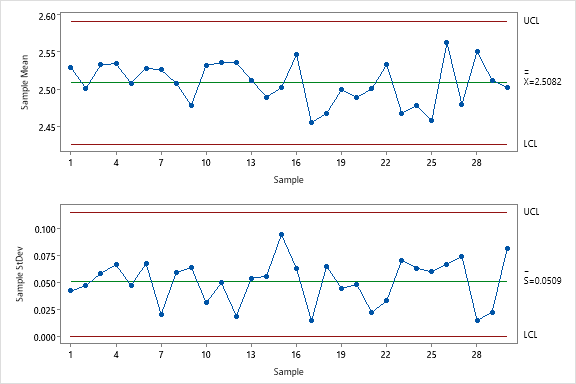
\includegraphics[width=0.75\textwidth]{Xbar_S_Paper.png}
\end{figure}


\item Una empresa que fabrica tarjetas de circuitos impresos desea evaluar si la implementaci\'on de un nuevo sistema de ensamblaje ha reducido el n\'umero de disconformidades. Se tomaron 50 mediciones, antes y después del cambio, para analizar los efectos.
\begin{center}
\begin{tabular}{|l|c|c|}
\hline
 & Antes & Después \\ 
\hline
Media muestral & 3.60 & 2.37 \\ 
\hline
Desviaci'on est'andar muestral & 1.09 & 1.62 \\ 
\hline
\end{tabular}
\end{center}
\begin{enumerate}
\item (15 pts) Calcula un intervalo de confianza de 90\% para el número medio de disconformidades antes del cambio.
\item (15 pts) ¿Existe suficiente evidencia para concluir que el número medio de disconformidades ha disminuido despu\'es del cambio? Usa un nivel de significancia de 0.05.
\end{enumerate}


\end{enumerate}
  
\newpage



\begin{center}
{\large Instituto Tecnol\'{o}gico y de Estudios Superiores de Monterrey \\
An\'alisis Estad\'stico de Datos } \\
Examen Argumentativo (Papel)
\end{center}

Nombre: \underline{\hspace*{.2in}}
Alberto Silva
\underline{\hspace*{.2in}} \quad Matr\'icula:\underline{\hspace*{.2in}}
A00000028
\underline{\hspace*{.2in}} \\

{\bf Instrucciones:} Lee con cuidado cada problema y escribe la soluci\'on
en tu hoja de respuesta. Incluye tu procedimiento que muestre c\'omo obtienes tu respuesta.  Respeta el c\'odigo de \'etica del curso y del Tecnol\'ogico de Monterrey y responde los ejercicios de manera individual sin ayuda externa o no autorizada.

\begin{enumerate}

\item Una empresa que fabrica l\'aminas de aluminio para la industria aeron\'autica necesita asegurar que el espesor de sus l\'aminas cumple con las especificaciones de $2.5 \pm 0.1$ mm. Se ha implementado una nueva maquinaria y se desea monitorear el espesor de las l\'aminas. Para ello, se han tomado muestras de tama\~no 4 cada hora y se gener\'o el diagrama que se muestra abajo.
\begin{enumerate}
\item (5 pts) Calcula la media y variabilidad del proceso (dentro de grupos).
\item (10 pts) Calcula los l\'imites de control para el espesor de las láminas.
\item (10 pts) Calcula el porcentaje de l\'aminas que cumplen con las especificaciones. Use los valores del inciso a) para calcular este porcentaje.
\end{enumerate}
\begin{figure}[h!]
\centering
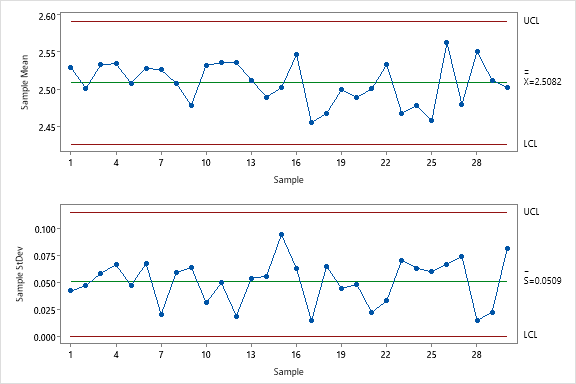
\includegraphics[width=0.75\textwidth]{Xbar_S_Paper.png}
\end{figure}


\item Una empresa que fabrica tarjetas de circuitos impresos desea evaluar si la implementaci\'on de un nuevo sistema de ensamblaje ha reducido el n\'umero de disconformidades. Se tomaron 50 mediciones, antes y después del cambio, para analizar los efectos.
\begin{center}
\begin{tabular}{|l|c|c|}
\hline
 & Antes & Después \\ 
\hline
Media muestral & 3.60 & 2.37 \\ 
\hline
Desviaci'on est'andar muestral & 1.09 & 1.62 \\ 
\hline
\end{tabular}
\end{center}
\begin{enumerate}
\item (15 pts) Calcula un intervalo de confianza de 90\% para el número medio de disconformidades antes del cambio.
\item (15 pts) ¿Existe suficiente evidencia para concluir que el número medio de disconformidades ha disminuido despu\'es del cambio? Usa un nivel de significancia de 0.05.
\end{enumerate}


\end{enumerate}
  
\newpage



\begin{center}
{\large Instituto Tecnol\'{o}gico y de Estudios Superiores de Monterrey \\
An\'alisis Estad\'stico de Datos } \\
Examen Argumentativo (Papel)
\end{center}

Nombre: \underline{\hspace*{.2in}}
Ximena Rojas
\underline{\hspace*{.2in}} \quad Matr\'icula:\underline{\hspace*{.2in}}
A00000029
\underline{\hspace*{.2in}} \\

{\bf Instrucciones:} Lee con cuidado cada problema y escribe la soluci\'on
en tu hoja de respuesta. Incluye tu procedimiento que muestre c\'omo obtienes tu respuesta.  Respeta el c\'odigo de \'etica del curso y del Tecnol\'ogico de Monterrey y responde los ejercicios de manera individual sin ayuda externa o no autorizada.

\begin{enumerate}

\item Una empresa que fabrica l\'aminas de aluminio para la industria aeron\'autica necesita asegurar que el espesor de sus l\'aminas cumple con las especificaciones de $2.5 \pm 0.1$ mm. Se ha implementado una nueva maquinaria y se desea monitorear el espesor de las l\'aminas. Para ello, se han tomado muestras de tama\~no 4 cada hora y se gener\'o el diagrama que se muestra abajo.
\begin{enumerate}
\item (5 pts) Calcula la media y variabilidad del proceso (dentro de grupos).
\item (10 pts) Calcula los l\'imites de control para la {\bf variabilidad} del espesor de las láminas.
\item (10 pts) Calcula el porcentaje de l\'aminas que tienen un espesor mayor a 2.6 mm. Use los valores del inciso a) para calcular este porcentaje.
\end{enumerate}
\begin{figure}[h!]
\centering
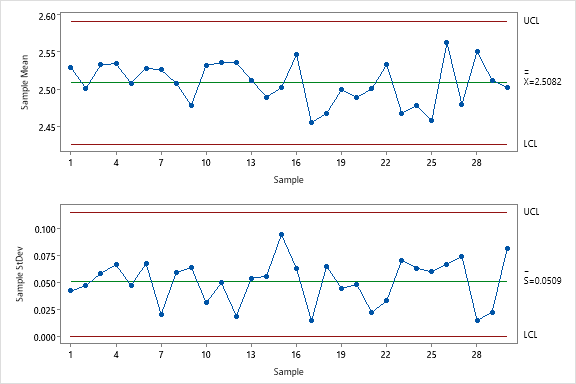
\includegraphics[width=0.75\textwidth]{Xbar_S_Paper.png}
\end{figure}


\item Una empresa que fabrica tarjetas de circuitos impresos desea evaluar si la implementaci\'on de un nuevo sistema de ensamblaje ha reducido el n\'umero de disconformidades. Se tomaron 50 mediciones, antes y después del cambio, para analizar los efectos.
\begin{center}
\begin{tabular}{|l|c|c|}
\hline
 & Antes & Después \\ 
\hline
Media muestral & 3.60 & 2.37 \\ 
\hline
Desviaci'on est'andar muestral & 1.09 & 1.62 \\ 
\hline
\end{tabular}
\end{center}
\begin{enumerate}
\item (15 pts) Calcula un intervalo de confianza de 90\% para el número medio de disconformidades antes del cambio.
\item (15 pts) ¿Existe suficiente evidencia para concluir que el número medio de disconformidades ha disminuido despu\'es del cambio? Usa un nivel de significancia de 0.05.
\end{enumerate}


\end{enumerate}
  
\newpage



\begin{center}
{\large Instituto Tecnol\'{o}gico y de Estudios Superiores de Monterrey \\
An\'alisis Estad\'stico de Datos } \\
Examen Argumentativo (Papel)
\end{center}

Nombre: \underline{\hspace*{.2in}}
Julio Zamora
\underline{\hspace*{.2in}} \quad Matr\'icula:\underline{\hspace*{.2in}}
A00000030
\underline{\hspace*{.2in}} \\

{\bf Instrucciones:} Lee con cuidado cada problema y escribe la soluci\'on
en tu hoja de respuesta. Incluye tu procedimiento que muestre c\'omo obtienes tu respuesta.  Respeta el c\'odigo de \'etica del curso y del Tecnol\'ogico de Monterrey y responde los ejercicios de manera individual sin ayuda externa o no autorizada.

\begin{enumerate}

\item Una empresa que fabrica l\'aminas de aluminio para la industria aeron\'autica necesita asegurar que el espesor de sus l\'aminas cumple con las especificaciones de $2.5 \pm 0.1$ mm. Se ha implementado una nueva maquinaria y se desea monitorear el espesor de las l\'aminas. Para ello, se han tomado muestras de tama\~no 4 cada hora y se gener\'o el diagrama que se muestra abajo.
\begin{enumerate}
\item (5 pts) Calcula la media y variabilidad del proceso (dentro de grupos).
\item (10 pts) Calcula los l\'imites de control para la {\bf variabilidad} del espesor de las láminas.
\item (10 pts) Calcula el porcentaje de l\'aminas que tienen un espesor mayor a 2.6 mm. Use los valores del inciso a) para calcular este porcentaje.
\end{enumerate}
\begin{figure}[h!]
\centering
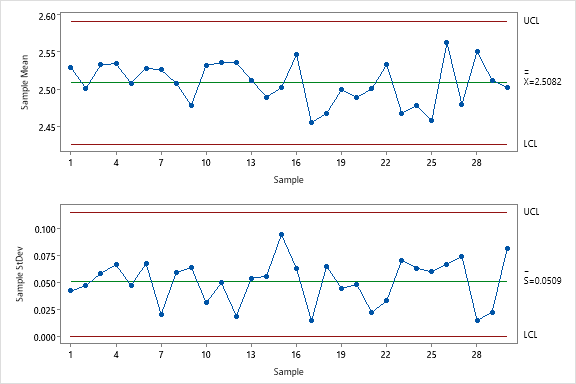
\includegraphics[width=0.75\textwidth]{Xbar_S_Paper.png}
\end{figure}


\item Una empresa que fabrica tarjetas de circuitos impresos desea evaluar si la implementaci\'on de un nuevo sistema de ensamblaje ha reducido el n\'umero de disconformidades. Se tomaron 50 mediciones, antes y después del cambio, para analizar los efectos.
\begin{center}
\begin{tabular}{|l|c|c|}
\hline
 & Antes & Después \\ 
\hline
Media muestral & 3.60 & 2.37 \\ 
\hline
Desviaci'on est'andar muestral & 1.09 & 1.62 \\ 
\hline
\end{tabular}
\end{center}
\begin{enumerate}
\item (15 pts) Calcula un intervalo de confianza de 90\% para el número medio de disconformidades antes del cambio.
\item (15 pts) ¿Existe suficiente evidencia para concluir que el número medio de disconformidades ha disminuido despu\'es del cambio? Usa un nivel de significancia de 0.05.
\end{enumerate}


\end{enumerate}
  
\newpage



\begin{center}
{\large Instituto Tecnol\'{o}gico y de Estudios Superiores de Monterrey \\
An\'alisis Estad\'stico de Datos } \\
Examen Argumentativo (Papel)
\end{center}

Nombre: \underline{\hspace*{.2in}}
Karina Villalobos
\underline{\hspace*{.2in}} \quad Matr\'icula:\underline{\hspace*{.2in}}
A00000031
\underline{\hspace*{.2in}} \\

{\bf Instrucciones:} Lee con cuidado cada problema y escribe la soluci\'on
en tu hoja de respuesta. Incluye tu procedimiento que muestre c\'omo obtienes tu respuesta.  Respeta el c\'odigo de \'etica del curso y del Tecnol\'ogico de Monterrey y responde los ejercicios de manera individual sin ayuda externa o no autorizada.

\begin{enumerate}

\item Una empresa que fabrica l\'aminas de aluminio para la industria aeron\'autica necesita asegurar que el espesor de sus l\'aminas cumple con las especificaciones de $2.5 \pm 0.1$ mm. Se ha implementado una nueva maquinaria y se desea monitorear el espesor de las l\'aminas. Para ello, se han tomado muestras de tama\~no 4 cada hora y se gener\'o el diagrama que se muestra abajo.
\begin{enumerate}
\item (5 pts) Calcula la media y variabilidad del proceso (dentro de grupos).
\item (10 pts) Calcula los l\'imites de control para la {\bf variabilidad} del espesor de las láminas.
\item (10 pts) Calcula el porcentaje de l\'aminas que tienen un espesor mayor a 2.6 mm. Use los valores del inciso a) para calcular este porcentaje.
\end{enumerate}
\begin{figure}[h!]
\centering
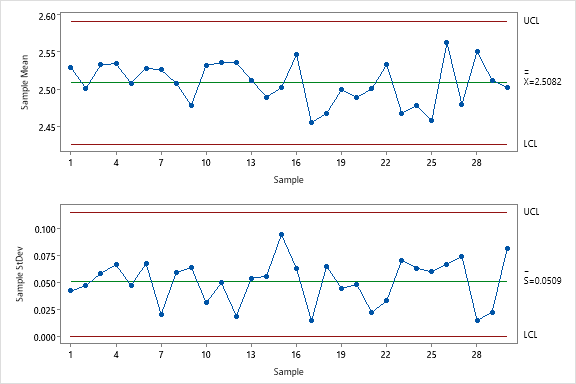
\includegraphics[width=0.75\textwidth]{Xbar_S_Paper.png}
\end{figure}


\item Una empresa que fabrica tarjetas de circuitos impresos desea evaluar si la implementaci\'on de un nuevo sistema de ensamblaje ha reducido el n\'umero de disconformidades. Se tomaron 50 mediciones, antes y después del cambio, para analizar los efectos.
\begin{center}
\begin{tabular}{|l|c|c|}
\hline
 & Antes & Después \\ 
\hline
Media muestral & 3.60 & 2.37 \\ 
\hline
Desviaci'on est'andar muestral & 1.09 & 1.62 \\ 
\hline
\end{tabular}
\end{center}
\begin{enumerate}
\item (15 pts) Calcula un intervalo de confianza de 90\% para el número medio de disconformidades antes del cambio.
\item (15 pts) ¿Existe suficiente evidencia para concluir que el número medio de disconformidades ha disminuido despu\'es del cambio? Usa un nivel de significancia de 0.05.
\end{enumerate}


\end{enumerate}
  
\newpage



\begin{center}
{\large Instituto Tecnol\'{o}gico y de Estudios Superiores de Monterrey \\
An\'alisis Estad\'stico de Datos } \\
Examen Argumentativo (Papel)
\end{center}

Nombre: \underline{\hspace*{.2in}}
Miguel Cervantes
\underline{\hspace*{.2in}} \quad Matr\'icula:\underline{\hspace*{.2in}}
A00000032
\underline{\hspace*{.2in}} \\

{\bf Instrucciones:} Lee con cuidado cada problema y escribe la soluci\'on
en tu hoja de respuesta. Incluye tu procedimiento que muestre c\'omo obtienes tu respuesta.  Respeta el c\'odigo de \'etica del curso y del Tecnol\'ogico de Monterrey y responde los ejercicios de manera individual sin ayuda externa o no autorizada.

\begin{enumerate}

\item Una empresa que fabrica l\'aminas de aluminio para la industria aeron\'autica necesita asegurar que el espesor de sus l\'aminas cumple con las especificaciones de $2.5 \pm 0.1$ mm. Se ha implementado una nueva maquinaria y se desea monitorear el espesor de las l\'aminas. Para ello, se han tomado muestras de tama\~no 4 cada hora y se gener\'o el diagrama que se muestra abajo.
\begin{enumerate}
\item (5 pts) Calcula la media y variabilidad del proceso (dentro de grupos).
\item (10 pts) Calcula los l\'imites de control para el espesor de las láminas.
\item (10 pts) Calcula el porcentaje de l\'aminas que cumplen con las especificaciones. Use los valores del inciso a) para calcular este porcentaje.
\end{enumerate}
\begin{figure}[h!]
\centering
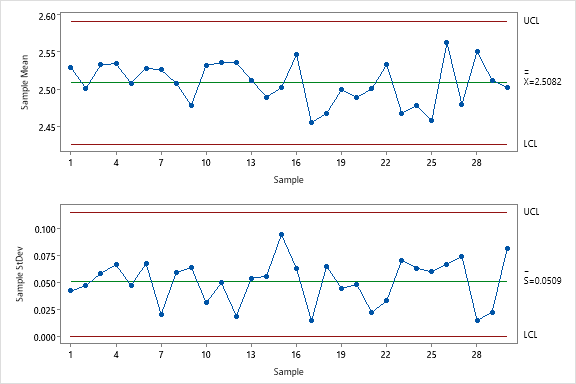
\includegraphics[width=0.75\textwidth]{Xbar_S_Paper.png}
\end{figure}


\item Una empresa que fabrica tarjetas de circuitos impresos desea evaluar si la implementaci\'on de un nuevo sistema de ensamblaje ha reducido el n\'umero de disconformidades. Se tomaron 50 mediciones, antes y después del cambio, para analizar los efectos.
\begin{center}
\begin{tabular}{|l|c|c|}
\hline
 & Antes & Después \\ 
\hline
Media muestral & 3.60 & 2.37 \\ 
\hline
Desviaci'on est'andar muestral & 1.09 & 1.62 \\ 
\hline
\end{tabular}
\end{center}
\begin{enumerate}
\item (15 pts) Calcula un intervalo de confianza de 90\% para el número medio de disconformidades antes del cambio.
\item (15 pts) ¿Existe suficiente evidencia para concluir que el número medio de disconformidades ha disminuido despu\'es del cambio? Usa un nivel de significancia de 0.05.
\end{enumerate}


\end{enumerate}
  
\newpage



\begin{center}
{\large Instituto Tecnol\'{o}gico y de Estudios Superiores de Monterrey \\
An\'alisis Estad\'stico de Datos } \\
Examen Argumentativo (Papel)
\end{center}

Nombre: \underline{\hspace*{.2in}}
Josué Miramontes
\underline{\hspace*{.2in}} \quad Matr\'icula:\underline{\hspace*{.2in}}
A00000033
\underline{\hspace*{.2in}} \\

{\bf Instrucciones:} Lee con cuidado cada problema y escribe la soluci\'on
en tu hoja de respuesta. Incluye tu procedimiento que muestre c\'omo obtienes tu respuesta.  Respeta el c\'odigo de \'etica del curso y del Tecnol\'ogico de Monterrey y responde los ejercicios de manera individual sin ayuda externa o no autorizada.

\begin{enumerate}

\item Una empresa que fabrica l\'aminas de aluminio para la industria aeron\'autica necesita asegurar que el espesor de sus l\'aminas cumple con las especificaciones de $2.5 \pm 0.1$ mm. Se ha implementado una nueva maquinaria y se desea monitorear el espesor de las l\'aminas. Para ello, se han tomado muestras de tama\~no 4 cada hora y se gener\'o el diagrama que se muestra abajo.
\begin{enumerate}
\item (5 pts) Calcula la media y variabilidad del proceso (dentro de grupos).
\item (10 pts) Calcula los l\'imites de control para la {\bf variabilidad} del espesor de las láminas.
\item (10 pts) Calcula el porcentaje de l\'aminas que tienen un espesor mayor a 2.6 mm. Use los valores del inciso a) para calcular este porcentaje.
\end{enumerate}
\begin{figure}[h!]
\centering
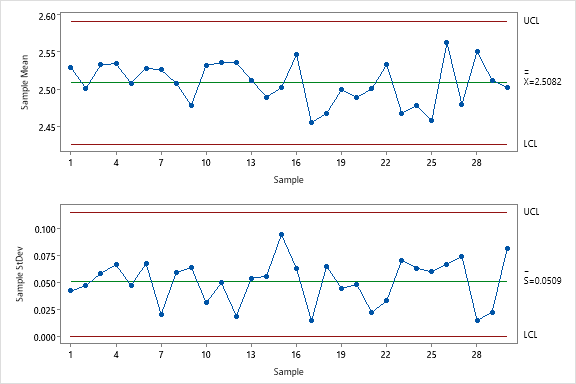
\includegraphics[width=0.75\textwidth]{Xbar_S_Paper.png}
\end{figure}


\item Una empresa que fabrica tarjetas de circuitos impresos desea evaluar si la implementaci\'on de un nuevo sistema de ensamblaje ha reducido el n\'umero de disconformidades. Se tomaron 50 mediciones, antes y después del cambio, para analizar los efectos.
\begin{center}
\begin{tabular}{|l|c|c|}
\hline
 & Antes & Después \\ 
\hline
Media muestral & 3.60 & 2.37 \\ 
\hline
Desviaci'on est'andar muestral & 1.09 & 1.62 \\ 
\hline
\end{tabular}
\end{center}
\begin{enumerate}
\item (15 pts) Calcula un intervalo de confianza de 90\% para el número medio de disconformidades antes del cambio.
\item (15 pts) ¿Existe suficiente evidencia para concluir que el número medio de disconformidades ha disminuido despu\'es del cambio? Usa un nivel de significancia de 0.05.
\end{enumerate}


\end{enumerate}
  
\newpage


\end{document}
